\documentclass[11pt,a4paper]{article}

% Packages
\usepackage[utf8]{inputenc}
\usepackage[T1]{fontenc}
\usepackage{lmodern}
\usepackage{amsmath,amssymb,amsthm}
\usepackage{graphicx}
\usepackage{xcolor}
\usepackage{hyperref}
\usepackage{natbib}
\usepackage{booktabs}
\usepackage{array}
\usepackage{multirow}
\usepackage{caption}
\usepackage{subcaption}
\usepackage{tikz}
\usetikzlibrary{shapes,arrows,positioning,calc,decorations.pathreplacing}
\usepackage{algorithm}
\usepackage{algorithmic}
\usepackage{enumitem}
\usepackage{geometry}
\geometry{margin=1in}
\usepackage{adjustbox}  % For auto-scaling tables

% Bibliography style
\bibliographystyle{unsrtnat}

% Title information
\title{\textbf{From Prediction to Design: A Paradigm Shift in AI-Driven Protein-Protein Interaction Research}}
\author{
\textbf{Author Names}$^{1,*}$\\
\\
$^1$Affiliation\\
$^*$Corresponding author
}
\date{}

\begin{document}

\maketitle

\begin{abstract}
\noindent
Protein-protein interactions (PPIs) form the molecular foundation of cellular life processes. Over the past two decades, computational methods for PPI analysis have primarily focused on \textit{prediction}---given protein information, inferring interaction properties. However, a fundamental paradigm shift is now underway: from ``predicting what will happen'' to ``designing what we want.'' This transformation is driven by breakthroughs in protein language models, diffusion models, and equivariant neural networks. In this review, we systematically analyze this paradigm shift, examining the technical foundations that enable it, the core tasks in the design era, and the challenges that lie ahead. We argue that this transition marks a fundamental change in how AI interfaces with biological discovery---moving from passive observation to active creation---with profound implications for drug discovery, synthetic biology, and our understanding of the protein universe.
\end{abstract}

\noindent\textbf{Keywords:} protein-protein interactions, deep learning, generative models, protein design, AlphaFold, diffusion models, protein language models

\vspace{1em}

% Table of Contents (for draft)
\tableofcontents
\newpage

% Main content sections
% Section 1: Introduction
% Word count target: ~900 words

\section{Introduction}
\label{sec:introduction}

Protein-protein interactions (PPIs) form the molecular foundation of cellular life. Virtually every biological process---signal transduction, immune response, metabolism, gene regulation---relies on proteins interacting with specific partners. The human interactome is estimated to contain 130,000--650,000 binary interactions~\cite{szklarczyk2021string}, with each protein engaging an average of 5--10 partners. Disease-associated mutations disproportionately affect interaction interfaces: Sahni et al.~\cite{sahni2015edgotype} demonstrated that approximately 60\% of disease mutations perturb at least one protein-protein interaction, and over 25\% result in complete loss of interactions. These findings establish PPIs as important molecular determinants of disease phenotypes and attractive therapeutic targets.

Over the past two decades, computational approaches to PPI research have primarily focused on \textit{prediction}: given protein sequences or structures, infer whether and how they interact. This prediction paradigm has produced remarkable successes. Methods like PIPR~\cite{chen2019pipr} and D-SCRIPT~\cite{sledzieski2021dscript} achieve high accuracy in predicting binary interactions from sequence alone. AlphaFold-Multimer~\cite{evans2022alphafoldmultimer} and AlphaFold 3~\cite{abramson2024alphafold3} predict the three-dimensional structures of protein complexes with unprecedented accuracy. These capabilities have accelerated interactome mapping and enabled structure-based analysis of interaction networks.

Yet a fundamental limitation constrains prediction methods: they can only describe what might happen, not create what we want to happen. For drug discovery and synthetic biology, the relevant question is not ``will these proteins interact?'' but ``how can we design proteins that interact the way we need?'' This shift from passive observation to active creation defines the emerging \textit{design paradigm}.

\subsection*{Why This Paradigm Shift Matters}

The transition from prediction to design represents more than methodological evolution---it constitutes what Thomas Kuhn termed a ``paradigm shift'' in scientific practice~\cite{kuhn1962structure}. In Kuhn's framework, paradigms define not only what questions scientists ask but what questions are considered meaningful. The prediction paradigm asks: ``What interactions exist in nature?'' The design paradigm asks: ``What interactions can we create?'' This reconceptualization opens investigation into regions of sequence-structure space that evolution never explored but that may contain superior therapeutic or industrial properties.

The practical significance is substantial. Traditional drug discovery---screening large compound libraries---identifies leads against approximately 15\% of potential targets, leaving the majority ``undruggable'' due to lack of suitable binding pockets or chemical matter. Protein-based therapeutics can engage flat protein surfaces inaccessible to small molecules, potentially expanding druggable target space several-fold. Similarly, synthetic biology currently relies on repurposing natural protein components; design capabilities would enable creation of signaling pathways and biosensors unconstrained by evolutionary history.

The economic implications are equally significant. Drug development costs, including failed candidates, are estimated at \$0.8--2.0 billion per approved therapeutic (median: \$1.3 billion) with timelines of 10--15 years~\cite{wouters2020cost}. Computational design could compress early-stage discovery from years to weeks, reducing both costs and time-to-patient. Early applications to SARS-CoV-2 demonstrated this potential: designed neutralizing proteins reached preclinical testing within 6--8 weeks rather than the years typically required for antibody development~\cite{watson2023rfdiffusion}.

\subsection*{Technological Foundations and Controversies}

This review argues that the field is undergoing a paradigm shift enabled by converging technological advances. Protein language models encode evolutionary and structural information at scale~\cite{rives2021esm1b,lin2023esm2}. Diffusion models generate novel protein structures conditioned on functional constraints~\cite{watson2023rfdiffusion,ingraham2023chroma}. Equivariant neural networks preserve geometric symmetries essential for accurate structure modeling~\cite{jing2021gvp,fuchs2020se3transformer}. Together, these technologies enable the creation of novel proteins with desired interaction properties.

However, the field is not without controversy. Critics note that success rates for de novo design remain modest (10--50\% depending on target) compared to natural protein engineering~\cite{bernett2024bias}. Questions persist about whether designed proteins will exhibit the stability, specificity, and lack of immunogenicity required for therapeutic use. Some argue that current ``design'' methods are better characterized as sophisticated optimization of natural scaffolds rather than true creation~\cite{kewalramani2023state}. This review addresses these critiques while presenting evidence that a paradigm shift, though incomplete and ongoing, represents a meaningful transformation in the field's capabilities.

The challenges are significant. Current methods struggle with dynamic interactions, multi-protein complexes, and generalization to novel targets. Evaluation remains problematic, with data leakage potentially inflating reported performance. The experimental validation bottleneck limits iterative improvement. These challenges define the research frontier that the field must address to realize the paradigm's full potential.

\subsection*{Article Structure}

This review provides a comprehensive analysis of this paradigm shift. Section~\ref{sec:prediction} examines the prediction paradigm's methods and limitations. Section~\ref{sec:design} traces the emergence of design capabilities. Section~\ref{sec:design_tasks} surveys core design tasks. Section~\ref{sec:technologies} details enabling technologies. Section~\ref{sec:challenges} discusses open challenges. Section~\ref{sec:applications} examines applications in therapeutics, synthetic biology, and basic research. Section~\ref{sec:future} offers perspectives on future directions, and Section~\ref{sec:conclusion} synthesizes key themes.

% ===== FIGURE 1: 范式转变概览图 =====
% 
% 图表类型: 双面板对比图 (Two-panel comparison diagram)
% 尺寸: 全页宽度 (single-column width for journal)
% 
% 【左面板 - 预测范式】
% 标题: "Prediction Paradigm"
% 
% 核心流程图 (从上到下的垂直流程):
% ┌─────────────────────────────────────────┐
% │         Input: Known Proteins           │
% │         (Sequences/Structures)          │
% └─────────────────┬───────────────────────┘
%                   ↓
% ┌─────────────────────────────────────────┐
% │    Computational Analysis/Prediction    │
% │    • Sequence similarity                │
% │    • Structure comparison               │
% │    • Machine learning classification    │
% │    (Methods: SVM, GNN, Transformers)    │
% └─────────────────┬───────────────────────┘
%                   ↓
% ┌─────────────────────────────────────────┐
% │    Output: Binary Classification        │
% │    "Will these proteins interact?"      │
% │    Answer: YES / NO                     │
% │    (Optional: Where? How strongly?)     │
% └─────────────────────────────────────────┘
%
% 特征标注:
% • 箭头: 灰色/蓝色
% • 问题标记: "Discovery Mode" 标签
% • 时间指示: "1980s-2020" (底部)
% • 关键词: "Understanding", "Analysis", "Classification"
%
% 【右面板 - 设计范式】
% 标题: "Design Paradigm"
%
% 核心流程图 (循环流程):
% ┌─────────────────────────────────────────┐
% │    Input: Design Goal/Target            │
% │    "What interaction do we WANT?"       │
% │    (Target structure + constraints)     │
% └─────────────────┬───────────────────────┘
%                   ↓
% ┌─────────────────────────────────────────┐
% │       Generative AI Design              │
% │    • Diffusion models (backbone)        │
% │    • Inverse folding (sequence)         │
% │    • Multi-objective optimization       │
% │    (Methods: RFdiffusion, AlphaProteo)  │
% └─────────────────┬───────────────────────┘
%                   ↓
% ┌─────────────────────────────────────────┐
% │    Output: Novel Protein Sequences      │
% │    "Here are proteins that WILL bind"   │
% │    (Candidate designs: 100s-1000s)      │
% └─────────────────┬───────────────────────┘
%                   ↓
% ┌─────────────────────────────────────────┐
% │    Validation & Iteration               │
% │    • Computational screening            │
% │    • Experimental testing               │
% │    • Feedback to improve design         │
% └─────────────────┬───────────────────────┘
%                   ↓ (loop back to top)
%
% 特征标注:
% • 箭头: 绿色/紫色
% • 循环标记: "Creative Mode" 标签
% • 时间指示: "2021-Present" (底部)
% • 关键词: "Creation", "Engineering", "Synthesis"
%
% 【中间分隔区域】
% 大箭头: 从左到右，标注 "PARADIGM SHIFT"
% 副标题: "From Analysis to Synthesis"
%
% 【底部对比表】(small table)
% ┌──────────────┬─────────────────┬──────────────────┐
% │ Aspect       │ Prediction      │ Design           │
% ├──────────────┼─────────────────┼──────────────────┤
% │ Goal         │ Understand      │ Create           │
% │ Question     │ "Will it?"      │ "How to make it?"│
% │ Output       │ Yes/No          │ New sequences    │
% │ Role of AI   │ Analyzer        │ Creator          │
% │ Key Methods  │ Classification  │ Generation       │
% └──────────────┴─────────────────┴──────────────────┘
%
% 颜色方案:
% • 背景: 白色
% • 预测范式: 蓝色系 (#4A90E2, #7BA3E2)
% • 设计范式: 绿色系 (#7ED321, #A8E6CF)
% • 箭头: 深灰色 (#4A4A4A)
% • 文字: 黑色 (#000000)
%
% 脚注: "Figure 1: The paradigm shift from prediction to design in AI-driven protein-protein interaction research. 
%        Left: The prediction paradigm analyzes existing proteins to determine interaction likelihood. 
%        Right: The design paradigm generates novel proteins with desired interaction properties."

\begin{figure}[t]
\centering
\resizebox{0.95\textwidth}{!}{%
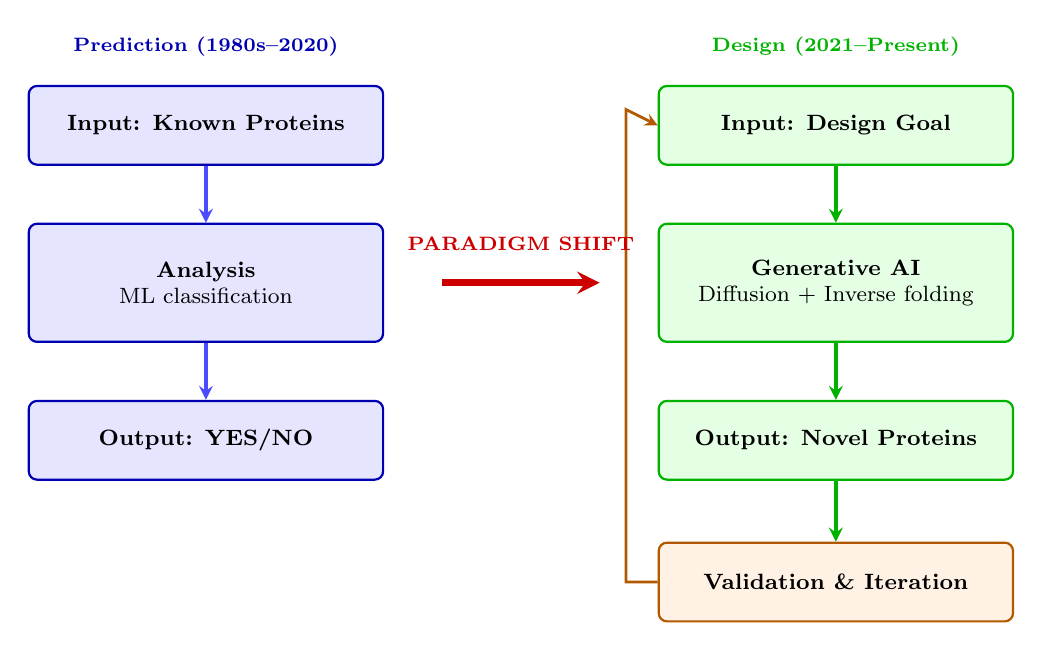
\begin{tikzpicture}[
    box/.style={rectangle, rounded corners=3pt, draw, minimum width=4.5cm, minimum height=1cm, align=center, font=\footnotesize},
    predbox/.style={box, fill=blue!10, draw=blue!70!black, line width=0.8pt},
    designbox/.style={box, fill=green!10, draw=green!70!black, line width=0.8pt},
    validatebox/.style={box, fill=orange!10, draw=orange!70!black, line width=0.8pt},
    arrow/.style={->, >=stealth, line width=1.2pt},
    predarrow/.style={arrow, blue!70},
    designarrow/.style={arrow, green!70!black}
]
% Prediction paradigm
\node[predbox] (p1) at (-4, 5) {\textbf{Input: Known Proteins}};
\node[predbox, minimum height=1.5cm] (p2) at (-4, 3) {\textbf{Analysis}\\ML classification};
\node[predbox] (p3) at (-4, 1) {\textbf{Output: YES/NO}};
\draw[predarrow] (p1) -- (p2);
\draw[predarrow] (p2) -- (p3);
\node[font=\scriptsize\bfseries, blue!70!black] at (-4, 6) {Prediction (1980s--2020)};
% Design paradigm
\node[designbox] (d1) at (4, 5) {\textbf{Input: Design Goal}};
\node[designbox, minimum height=1.5cm] (d2) at (4, 3) {\textbf{Generative AI}\\Diffusion + Inverse folding};
\node[designbox] (d3) at (4, 1) {\textbf{Output: Novel Proteins}};
\node[validatebox] (d4) at (4, -0.8) {\textbf{Validation \& Iteration}};
\draw[designarrow] (d1) -- (d2);
\draw[designarrow] (d2) -- (d3);
\draw[designarrow] (d3) -- (d4);
\draw[orange!70!black, ->, >=stealth, line width=1pt] (d4.west) -- ++(-0.4, 0) -- ++(0, 6) -- (d1.west);
\node[font=\scriptsize\bfseries, green!70!black] at (4, 6) {Design (2021--Present)};
% Center arrow
\draw[red!80!black, ->, >=stealth, line width=2.5pt] (-1, 3) -- (1, 3);
\node[font=\scriptsize\bfseries, red!80!black] at (0, 3.5) {PARADIGM SHIFT};
\end{tikzpicture}
}
\caption{The paradigm shift from prediction to design in AI-driven PPI research. \textbf{Left panel (Prediction Paradigm, 1980s--2020):} Traditional computational approaches analyze known protein sequences and structures to predict interaction likelihood (YES/NO). Blue color scheme indicates analytical methods including machine learning classification and structure comparison. \textbf{Right panel (Design Paradigm, 2021--present):} Modern AI-driven approaches generate novel protein sequences with desired interaction properties through iterative design-test cycles. Green color scheme indicates generative methods including diffusion models and inverse folding. The validation loop (orange) reflects the critical role of experimental feedback in refining designs---computational predictions require physical validation to confirm binding affinity, specificity, and stability. \textbf{Center:} Red arrow marks the paradigm transition, enabled by breakthroughs in protein language models, structure prediction (AlphaFold2, RoseTTAFold), and generative AI.}
\label{fig:paradigm}
\end{figure}

% Section 2: The Prediction Paradigm: Methods and Limitations
% Word count target: ~1500 words

\section{The Prediction Paradigm: Methods and Limitations}
\label{sec:prediction}

Before the emergence of generative design approaches, the field of computational protein-protein interaction (PPI) research was dominated by what we term the \textit{prediction paradigm}---the goal of inferring whether, where, and how strongly proteins interact based on their sequences or structures. This paradigm has produced remarkable successes but also faces fundamental limitations that motivated the shift toward design-oriented approaches.

\subsection{Task Taxonomy and Methodological Overview}
\label{subsec:tasks}

PPI prediction encompasses a heterogeneous family of tasks that differ in their inputs, outputs, and computational strategies (Table~\ref{tab:ppi_tasks}). The most fundamental task is \textit{binary classification}: given two protein sequences, predict whether they physically interact. This task underlies large-scale interactome mapping efforts and has been the primary benchmark for method development.

\begin{table}[h]
\centering
\caption{Taxonomy of PPI prediction tasks}
\label{tab:ppi_tasks}
\begin{adjustbox}{max width=\textwidth}
\begin{tabular}{@{}llll@{}}
\toprule
\textbf{Task} & \textbf{Input} & \textbf{Output} & \textbf{Representative Methods} \\
\midrule
Binary classification & Sequence pairs & Interaction (yes/no) & PIPR~\cite{chen2019pipr}, D-SCRIPT~\cite{sledzieski2021dscript} \\
Network inference & Protein set & Interaction network & STRING~\cite{szklarczyk2021string}, GNN-PPI~\cite{lv2021gnnppi} \\
Binding site prediction & Single protein & Interface residues & MaSIF~\cite{gainza2020masif}, GraphPPIS~\cite{cao2022graphppis} \\
Affinity prediction & Complex + mutation & $\Delta\Delta G$ & FoldX~\cite{guerois2005foldx}, SKEMPI~\cite{jankauskaite2019skempi2} \\
Complex structure & Sequence pairs & 3D coordinates & AF-Multimer~\cite{evans2022alphafoldmultimer}, DiffDock-PP~\cite{ketata2023diffdockpp} \\
\bottomrule
\end{tabular}
\end{adjustbox}
\end{table}

Beyond binary classification, \textit{binding site prediction} aims to identify which residues mediate the interaction---critical information for drug design and mutagenesis studies~\cite{ortegon2020binding}. \textit{Affinity prediction} quantifies binding strength changes upon mutation, essential for understanding disease variants and optimizing therapeutic proteins. \textit{Complex structure prediction}---the most recent breakthrough---generates the full three-dimensional arrangement of interacting proteins.

\subsection{Sequence-Based Prediction Methods}
\label{subsec:sequence}

Sequence-based methods have evolved through three distinct generations, each representing a fundamental shift in how protein information is represented and processed.

\subsubsection{The Hand-Crafted Feature Era (2001--2015)}

Early methods relied on manually designed features extracted from amino acid sequences. Bock and Gough~\cite{bock2001predicting} pioneered this approach by using support vector machines (SVMs) with physicochemical properties, achieving the first systematic machine learning prediction of PPIs from primary structure. Shen et al.~\cite{shen2007predicting} introduced the \textit{conjoint triad} method, which grouped amino acids into seven classes based on dipoles and side-chain volumes, representing protein pairs as 343-dimensional vectors. This method achieved approximately 84\% accuracy on human PPIs and became widely adopted.

Guo et al.~\cite{guo2008using} advanced this line of work by introducing the \textit{auto-covariance} (AC) descriptor, which captures interactions between residues at varying sequence distances---overcoming the limitation of conjoint triad's nearest-neighbor assumption. Their SVM-based approach achieved 88\% accuracy on yeast PPIs. Ben-Hur and Noble~\cite{benhur2005kernel} developed pairwise kernel methods that enabled SVMs to operate directly on protein pairs without explicit feature concatenation.

A parallel tradition leveraged evolutionary information through position-specific scoring matrices (PSSMs). You et al.~\cite{you2017pssm} combined PSSM-derived features with discriminative vector machines, demonstrating that evolutionary conservation patterns carry strong interaction signals.

\subsubsection{The Deep Learning Era (2016--2020)}

The introduction of deep learning fundamentally changed PPI prediction by enabling automatic feature learning. DeepPPI~\cite{chen2017deepppi} was among the first to apply deep neural networks to this task, using separate networks for each protein followed by a fusion layer. Their approach achieved over 97\% AUC on benchmark datasets, significantly outperforming SVM-based methods.

DPPI~\cite{hashemifar2018dppi} introduced a Siamese convolutional architecture with random projection modules that efficiently explore motif combinations between protein pairs. This design enabled training on over 100,000 PPIs while maintaining computational efficiency. PIPR~\cite{chen2019pipr} combined residual networks with recurrent convolutions in a Siamese framework, unifying binary classification, interaction type prediction, and binding affinity estimation in a single architecture.

\subsubsection{The Pre-trained Model Era (2021--Present)}

The most recent advancement comes from protein language models (PLMs). D-SCRIPT~\cite{sledzieski2021dscript} leveraged pre-trained representations from ESM~\cite{rives2021esm1b} to infer inter-protein contact maps as an intermediate structural output, improving cross-species generalizability since structure is more conserved than sequence. Topsy-Turvy~\cite{singh2022topsyturvy} integrated sequence-based ``bottom-up'' predictions with network topology ``top-down'' information using multi-scale deep learning.

Graph neural networks (GNNs) have emerged as a powerful approach for PPI prediction, leveraging both network topology and protein features. GNN-PPI~\cite{lv2021gnnppi} demonstrated that learning unknown correlations in protein-protein interactions with deep graph neural networks achieves superior performance on network completion tasks. HIGH-PPI~\cite{tang2021high} introduced a high-order graph neural network that captures complex interaction patterns beyond pairwise relationships. DeepRank-GNN~\cite{bryant2022deeprank} introduced a framework to learn patterns in protein-protein interfaces directly from structural graphs.

More recent methods have developed specialized architectures. TAGPPI~\cite{xie2022tagppi} incorporated predicted structural information into sequence-based predictions. TUnA~\cite{gehring2024tuna} introduced uncertainty quantification to transformer-based PPI prediction. The recent PLM-interact~\cite{zhao2025plminteract} and MINT~\cite{ullanat2025mint} models extend PLMs specifically for interaction modeling, learning the ``language of protein interactions'' from large-scale interaction datasets such as BioPlex~\cite{huttlin2021bioplex} and IntAct~\cite{orchard2014intact}.

\subsection{Structure-Based Prediction Methods}
\label{subsec:structure}

Structure-based methods leverage three-dimensional information, either from experimental structures or computational predictions.

\subsubsection{Traditional Docking Approaches}

Classical protein-protein docking addresses the inverse problem: given two protein structures, predict their bound complex. HADDOCK~\cite{dominguez2003haddock} introduced information-driven docking by incorporating biochemical or biophysical constraints. ZDOCK~\cite{pierce2014zdock} uses fast Fourier transforms for efficient shape complementarity scoring. ClusPro~\cite{kozakov2017cluspro} provides automated docking through clustering of low-energy conformations. HDOCK~\cite{yan2020hdock} combines template-based and free docking strategies for protein-protein and protein-nucleic acid complexes. GalaxyTongDock~\cite{baek2023galaxytongdock} enables symmetric and asymmetric ab initio docking with improved energy parameters. HDOCK~\cite{yan2020hdock} integrates template-based and free docking with a hybrid scoring function, while GalaxyTongDock~\cite{baek2023galaxytongdock} supports both symmetric and asymmetric docking with improved energy parameters.

These methods assume rigid or semi-flexible structures and typically generate multiple candidate poses that must be ranked. Their accuracy depends heavily on the quality of input structures and the availability of constraint information.

\subsubsection{Interface Prediction from Structure}

Surface-based deep learning methods predict binding interfaces directly from molecular surfaces. MaSIF~\cite{gainza2020masif} applied geometric deep learning to protein surfaces, learning fingerprints that encode interaction propensities. GraphPPIS~\cite{cao2022graphppis} used graph convolutional networks on protein structure graphs. dMaSIF~\cite{sverrisson2021dmasif} replaced expensive mesh generation with point-cloud operators, achieving 10--100$\times$ speedups.

PeSTo~\cite{gao2023pestoppi} introduced a parameter-free geometric transformer that processes atomic coordinates without requiring sequence profiles, enabling efficient prediction across the growing ``foldome'' of predicted structures.

\subsubsection{End-to-End Complex Prediction}

The most dramatic recent advance is end-to-end prediction of complex structures from sequences alone. AlphaFold-Multimer~\cite{evans2022alphafoldmultimer} extended AlphaFold2's architecture~\cite{jumper2021alphafold} to multi-chain prediction, achieving breakthrough accuracy on many protein complexes. AlphaFold 3~\cite{abramson2024alphafold3} further generalized to arbitrary molecular assemblies including proteins, nucleic acids, and small molecules using a diffusion-based architecture.

DiffDock-PP~\cite{ketata2023diffdockpp} demonstrated the applicability of diffusion models to protein-protein docking, treating pose generation as a generative process rather than optimization.

\subsection{Fundamental Limitations of the Prediction Paradigm}
\label{subsec:limitations}

Despite remarkable progress, the prediction paradigm faces four fundamental limitations that motivated the emergence of design-oriented approaches.

\subsubsection{Data Dependence}

Prediction models are fundamentally data-dependent: they learn statistical patterns from known interactions and struggle to extrapolate to novel interaction types~\cite{kewalramani2023state}. Training data is heavily biased toward model organisms (human, yeast, mouse), limiting applicability to understudied proteins. Negative sample construction introduces systematic bias---randomly paired proteins may not represent true non-interactors~\cite{smialowski2010negatome}.

The Negatome database~\cite{blohm2014negatome2} addressed this by curating experimentally verified non-interacting pairs, but coverage remains limited. Prediction accuracy degrades significantly for proteins dissimilar from training examples, as demonstrated by the C1/C2/C3 difficulty classification framework~\cite{park2015ppi}.

\subsubsection{The Evaluation Crisis}

A critical 2024 study by Bernett et al.~\cite{bernett2024bias} revealed that many reported high accuracies result from data leakage---train-test overlap at the sequence similarity level. When rigorous cross-validation protocols prevent such leakage, model performance drops substantially. This finding suggests that many ``successful'' methods primarily learn to recognize sequence similarity to known interactors rather than genuine interaction features.

Benchmark datasets themselves suffer from incompleteness and bias. STRING~\cite{szklarczyk2021string} integrates multiple evidence sources with confidence scoring, but physical versus functional interactions are conflated. SKEMPI~\cite{jankauskaite2019skempi2} provides standardized affinity measurements but covers only a small fraction of known interactions. Benchmarking studies of AlphaFold~\cite{bryant2022benchmarking} have revealed important determinants of prediction accuracy for protein complexes.

\subsubsection{Passive Discovery Mode}

Prediction methods answer ``\textit{will} these proteins interact?'' rather than ``\textit{how can we make} them interact?'' For drug discovery and protein engineering, researchers need constructive capabilities: given a target protein, design a binder with desired properties~\cite{trepte2024ai}. The prediction paradigm provides no direct pathway from prediction to intervention.

This limitation is particularly acute for therapeutic applications. If a disease-associated PPI lacks a natural interactor that can serve as a drug, prediction methods offer no solution~\cite{feng2022frameworks}. Recent comprehensive reviews have highlighted this gap: while PPI prediction methods achieve increasingly accurate classification, they cannot directly guide the design of novel binding proteins with specified affinities and specificities~\cite{kewalramani2023state}. What is needed is the ability to \textit{create} new interactions de novo---precisely the capability that generative design approaches aim to provide.

\subsubsection{Static Assumptions}

Most PPI prediction methods treat interactions as static entities---a pair of proteins either interacts or does not. This assumption ignores the dynamic nature of the interactome~\cite{mcgary2010dynamic}. Interactions can be tissue-specific, condition-dependent, or transient. Time-resolved interaction networks remain largely inaccessible to current computational approaches.

AlphaFold-based methods~\cite{abramson2024alphafold3, evans2022alphafoldmultimer} predict static complex structures but do not capture conformational dynamics or binding kinetics. The integration of dynamical information from molecular dynamics or NMR ensembles into deep learning frameworks remains an open challenge.

\vspace{1em}
\noindent
These limitations collectively define the boundary of the prediction paradigm and motivate the paradigm shift toward generative design---the subject of Section~\ref{sec:design}.

% Section 3: The Emergence of Design Paradigm (Revised)
% Target: ~1,500 words

\section{The Emergence of Design Paradigm}
\label{sec:design}

% ===== FIGURE 2: 技术演进时间线 =====
%
% 图表类型: 横向时间线图 (Horizontal timeline diagram)
% 尺寸: 全页宽度 (single-column width)
%
% 【主时间轴】
% 横向时间线: 2018 ──── 2020 ──── 2022 ──── 2024 ──── 2025
%
% 【技术里程碑标注】(在时间轴上下交替标注)
%
% 2018-2019 (预测范式成熟期):
% ┌────────────────────────────────┐
% │ AlphaFold (2018)               │  ↑ Above timeline
% │ CASP13 breakthrough             │
% │ First deep learning structure  │
% └────────────────────────────────┘
%
% 2020-2021 (预测范式突破):
% ┌────────────────────────────────┐  ↓ Below timeline
% │ AlphaFold2 (Jul 2021)          │
% │ "Solving" protein folding      │
% │ Nature publication             │
% └────────────────────────────────┘
% ┌────────────────────────────────┐
% │ RoseTTAFold (2021)             │  ↑ Above
% │ Three-track network            │
% │ Science publication            │
% └────────────────────────────────┘
% ┌────────────────────────────────┐
% │ ESM-1b (2021)                  │  ↓ Below
% │ 650M parameter PLM             │
% │ Language models for proteins   │
% └────────────────────────────────┘
%
% 2022 (设计工具出现):
% ┌────────────────────────────────┐
% │ ProteinMPNN (Sep 2022)         │  ↑ Above
% │ Inverse folding                │
% │ 52.4% sequence recovery        │
% │ Science publication            │
% └────────────────────────────────┘
% ┌────────────────────────────────┐
% │ ESM-2/ESMFold (2022)           │  ↓ Below
% │ 15B parameters                 │
% │ 60× faster than AF2            │
% └────────────────────────────────┘
% ┌────────────────────────────────┐
% │ AlphaFold-Multimer (2022)      │  ↑ Above
% │ Complex prediction             │
% │ 67% interface accuracy         │
% └────────────────────────────────┘
%
% 2023 (生成式设计突破):
% ┌────────────────────────────────┐
% │ RFdiffusion (Feb 2023)         │  ↓ Below
% │ Diffusion for design           │
% │ Cryo-EM validated              │
% │ Nature publication             │
% └────────────────────────────────┘
% ┌────────────────────────────────┐
% │ Chroma (2023)                  │  ↑ Above
% │ Polymer statistics             │
% │ 4000 AA generation             │
% └────────────────────────────────┘
% ┌────────────────────────────────┐
% │ FrameDiff (2023)               │  ↓ Below
% │ SE(3) diffusion                │
% └────────────────────────────────┘
%
% 2024 (高级设计能力):
% ┌────────────────────────────────┐
% │ AlphaFold 3 (May 2024)         │  ↑ Above
% │ Multimodal complexes           │
% │ Diffusion architecture         │
% │ Nature publication             │
% └────────────────────────────────┘
% ┌────────────────────────────────┐
% │ AlphaProteo (Sep 2024)         │  ↓ Below
% │ High-affinity binders          │
% │ 3-300× success rate            │
% │ Nanomolar affinities           │
% └────────────────────────────────┘
% ┌────────────────────────────────┐
% │ RFdiffusionAA (2024)           │  ↑ Above
% │ Small molecule binding         │
% │ Cofactor design                │
% └────────────────────────────────┘
%
% 【阶段分隔线】
% • 2018-2021: "PREDICTION ERA" (蓝色背景区域)
% • 2022-2025: "DESIGN ERA" (绿色背景区域)
% • 在2021-2022之间画粗虚线，标注 "PARADIGM SHIFT"
%
% 【技术类型颜色编码】
% • 结构预测 (蓝色圆点): AlphaFold, RoseTTAFold, ESMFold
% • 语言模型 (紫色圆点): ESM-1b, ESM-2
% • 序列设计 (橙色圆点): ProteinMPNN, ESM-IF1
% • 生成设计 (绿色圆点): RFdiffusion, Chroma, AlphaProteo
%
% 【图例】
% ┌──────────────────────────────────┐
% │ ● 结构预测 (Structure)           │
% │ ● 语言模型 (PLM)                 │
% │ ● 序列设计 (Sequence Design)     │
% │ ● 生成设计 (Generative Design)   │
% └──────────────────────────────────┘
%
% 颜色方案:
% • 时间轴: 深灰色 (#4A4A4A), 粗线 3pt
% • 预测时代背景: 浅蓝色 (#E3F2FD), 透明度30%
% • 设计时代背景: 浅绿色 (#E8F5E9), 透明度30%
% • 分隔线: 红色虚线 (#F44336)
%
% 脚注: "Figure 2: Timeline of major technical breakthroughs in AI-driven protein research (2018-2024). 
%        The paradigm shift from prediction to design occurred around 2021-2022, marked by the emergence 
%        of generative methods capable of creating novel protein sequences and structures."

\begin{figure}[t]
\centering
\resizebox{0.95\textwidth}{!}{%
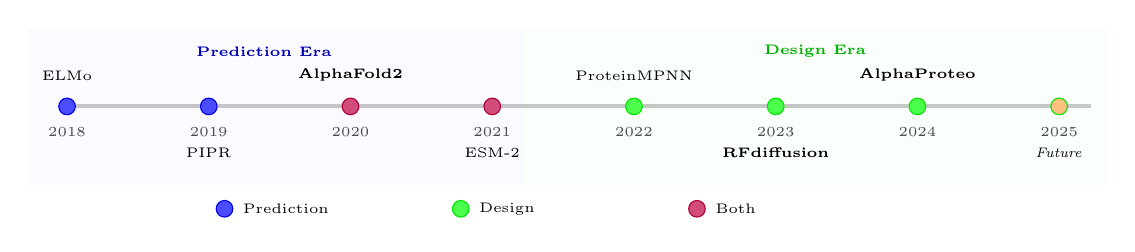
\begin{tikzpicture}[
    milestone/.style={circle, minimum size=6pt, inner sep=0pt},
    predmile/.style={milestone, fill=blue!70, draw=blue!90!black},
    designmile/.style={milestone, fill=green!70, draw=green!90!black},
    bothmile/.style={milestone, fill=purple!70, draw=purple!90!black}
]
% Timeline
\draw[line width=1.5pt, gray!60] (0, 0) -- (13, 0);
% Year markers
\foreach \x/\y in {0/2018, 1.8/2019, 3.6/2020, 5.4/2021, 7.2/2022, 9/2023, 10.8/2024, 12.6/2025} {
    \draw[gray!60] (\x, -0.1) -- (\x, 0.1);
    \node[font=\tiny, below] at (\x, -0.15) {\y};
}
% Phase backgrounds
\fill[blue!5, opacity=0.3] (-0.5, -1) rectangle (5.8, 1);
\fill[green!5, opacity=0.3] (5.8, -1) rectangle (13.2, 1);
\node[font=\tiny\bfseries, blue!70!black] at (2.5, 0.7) {Prediction Era};
\node[font=\tiny\bfseries, green!70!black] at (9.5, 0.7) {Design Era};
% Milestones
\node[predmile] at (0, 0) {};
\node[font=\tiny, above, align=center] at (0, 0.2) {ELMo};
\node[predmile] at (1.8, 0) {};
\node[font=\tiny, below, align=center] at (1.8, -0.4) {PIPR};
\node[bothmile] at (3.6, 0) {};
\node[font=\tiny, above, align=center] at (3.6, 0.2) {\textbf{AlphaFold2}};
\node[bothmile] at (5.4, 0) {};
\node[font=\tiny, below, align=center] at (5.4, -0.4) {ESM-2};
\node[designmile] at (7.2, 0) {};
\node[font=\tiny, above, align=center] at (7.2, 0.2) {ProteinMPNN};
\node[designmile] at (9, 0) {};
\node[font=\tiny, below, align=center] at (9, -0.4) {\textbf{RFdiffusion}};
\node[designmile] at (10.8, 0) {};
\node[font=\tiny, above, align=center] at (10.8, 0.2) {\textbf{AlphaProteo}};
\node[designmile, fill=orange!50] at (12.6, 0) {};
\node[font=\tiny, below, align=center] at (12.6, -0.4) {\textit{Future}};
% Legend
\node[predmile, label=right:{\tiny Prediction}] at (2, -1.3) {};
\node[designmile, label=right:{\tiny Design}] at (5, -1.3) {};
\node[bothmile, label=right:{\tiny Both}] at (8, -1.3) {};
\end{tikzpicture}
}
\caption{Timeline of major technical breakthroughs in AI-driven protein research (2018--2025). The paradigm shift from prediction to design occurred around 2021--2022, marked by the emergence of generative methods capable of creating novel proteins rather than merely analyzing existing ones. \textbf{Milestones shown in bold} (AlphaFold2, RFdiffusion, AlphaProteo) represent transformative advances with extensive experimental validation. \textbf{Color coding:} Blue dots indicate prediction-focused methods that analyze known proteins; green dots indicate design-focused methods that generate novel proteins; purple dots indicate methods spanning both paradigms. The shaded background regions delineate the Prediction Era (2018--2021, characterized by structure prediction breakthroughs) from the Design Era (2022--present, characterized by generative capabilities). The ``Future'' milestone (2025) reflects ongoing development of next-generation systems combining improved accuracy with enhanced computational efficiency.}
\label{fig:timeline}
\end{figure}

In 2021, DeepMind's AlphaFold2 achieved what many considered the ``grand challenge'' of computational biology: predicting protein structures from amino acid sequences with near-experimental accuracy~\citep{jumper2021alphafold}. Just two years later, researchers demonstrated something that would have seemed impossible a decade earlier: designing entirely new proteins that had never existed in nature, validated by cryo-EM structures showing atomic-level agreement with computational models~\citep{watson2023rfdiffusion}. This transition---from predicting what \textit{exists} to creating what \textit{should exist}---represents a fundamental paradigm shift in how artificial intelligence interfaces with protein science.

\subsection{Technical Drivers of the Paradigm Shift}
\label{subsec:drivers}

The emergence of the design paradigm was not a singular event but the convergence of multiple technological breakthroughs occurring between 2021 and 2024: structure prediction advances, generative models for proteins, scaled protein language models, and equivariant neural networks.

\subsubsection{Breakthroughs in Structure Prediction}

AlphaFold2's resolution of the protein folding problem~\citep{jumper2021alphafold} provided the foundation upon which protein design could be built. RoseTTAFold~\citep{baek2021rosettafold}, developed concurrently and published in the same year, demonstrated an alternative three-track architecture that achieved comparable accuracy with different computational trade-offs. The subsequent extension to multimeric complexes through AlphaFold-Multimer~\citep{evans2022alphafoldmultimer} and RoseTTAFold2~\citep{baek2023rosettafold2} expanded the scope to protein-protein interfaces, achieving correct interface prediction for 67\% of heterodimeric complexes. The significance of these advances for design is twofold: structure prediction provides a validation mechanism for designed proteins, and the underlying architectures contain learned representations that can be repurposed for generation. The Invariant Point Attention (IPA) mechanism introduced in AlphaFold2 has become a foundational architectural element in subsequent design systems. AlphaFold 3~\citep{abramson2024alphafold3} extended this capability further to complexes containing proteins, nucleic acids, small molecules, and ions.

\subsubsection{Introduction of Generative Models}

Diffusion models achieved breakthrough performance in image generation before being adapted to the protein domain. The fundamental principle underlying diffusion models is learning to reverse a gradual noising process: given a data distribution (valid protein structures), the forward process progressively adds Gaussian noise until the structure becomes random noise. The reverse process learns to denoise, iteratively recovering structure from noise.

For protein design, the key insight was recognizing that protein backbone conformations can be represented as SE(3) objects---3D structures with rotational and translational symmetries. SE(3) diffusion models~\citep{yim2023se3diffusion} operate directly on the manifold of rigid body frames, where each residue is represented by its position and orientation in 3D space. The denoising network must therefore be equivariant to rotations and translations, maintaining consistency regardless of the coordinate frame. FrameDiff demonstrated this approach could generate diverse, designable protein backbones without relying on pretrained structure prediction networks.

RFdiffusion~\citep{watson2023rfdiffusion} took a different approach by fine-tuning the pretrained RoseTTAFold network as a denoising model. This transfer learning strategy proved highly effective: RoseTTAFold's learned representations of protein structure provided a strong initialization for the generative task, reducing training time and improving sample quality. RFdiffusion conditions generation on partial structures (motifs, functional sites) or target proteins (for binder design), enabling targeted design rather than unconditional generation.

Chroma~\citep{ingraham2023chroma} was designed from the ground up as a generative model with a diffusion process that explicitly respects polymer conformational statistics. By incorporating physical constraints during training, Chroma generates proteins that satisfy both learned statistical patterns and physical plausibility. The system demonstrated generation of proteins up to 4,000 amino acids---far exceeding the typical 100-300 residue range of earlier methods.

An alternative to diffusion is flow matching, which learns deterministic trajectories through the space of protein structures rather than stochastic denoising paths. FoldFlow~\citep{bose2023foldflow} demonstrated that SE(3) flow matching can achieve comparable sample quality to diffusion while potentially offering better computational efficiency and mode coverage. However, flow-based approaches currently lag diffusion models in practical protein design applications, with fewer published experimental validations.

These generative approaches share common advantages: controllable generation through conditioning on specific constraints such as binding sites or symmetry requirements, natural production of diverse candidate structures for design space exploration, and learning the distribution of valid structures directly from data without hand-crafted energy functions. DiffDock-PP~\citep{ketata2023diffdockpp} adapted diffusion to protein-protein docking, treating pose generation as a generative process rather than optimization and achieving 44\% sampling success compared to 8\% for baselines.

\subsubsection{Scaling of Protein Language Models}

Protein language models (PLMs) learn meaningful protein representations through self-supervised pretraining on large sequence databases. ESM-1b~\citep{rives2021esm1b} demonstrated that transformer models capture evolutionary, structural, and functional information from sequence alone. ESM-2~\citep{lin2023esm2}, scaled to 15 billion parameters, achieved atomic-level structure prediction directly from sequence, with ESMFold running 60$\times$ faster than AlphaFold2. ProtTrans~\citep{elnaggar2021prottrans} established that encoder-only models outperform encoder-decoder architectures for protein understanding tasks.

These models provide a learned prior over protein sequences---encoding what sequences are likely to fold into stable, functional proteins. SaProt~\citep{su2024saprot} advanced this by introducing a structure-aware vocabulary that combines amino acid tokens with structural tokens. MINT~\citep{ullanat2025mint} and PLM-interact~\citep{zhao2025plminteract} extended PLMs specifically for PPI tasks, training on protein sets to model interaction propensities contextually.

\subsubsection{Development of Equivariant Neural Networks}

Equivariant neural networks process 3D geometric data while respecting physical symmetries, addressing the challenge that protein function depends on 3D structure but the same structure can be represented in any rotated or translated coordinate frame. This property is critical for protein design: a generated protein's validity should not depend on the arbitrary coordinate system in which it was generated.

SE(3)-Transformers~\citep{fuchs2020se3transformer} introduced attention mechanisms equivariant to 3D rotations and translations. The key architectural innovation is ensuring that attention weights depend only on relative positions and orientations---quantities invariant to global rotations---while the output features transform appropriately under coordinate changes. This equivariance-by-construction eliminates the need for data augmentation to cover all possible orientations, improving sample efficiency and generalization.

Geometric Vector Perceptrons (GVPs)~\citep{jing2021gvp} provided a simpler but equally effective approach through scalar-vector separation. Each node in the protein graph maintains both scalar features (amino acid type, biochemical properties) and vector features (spatial orientations, directional interactions). Message passing operates on both: scalar messages aggregate through standard attention or summation, while vector messages aggregate through rotation-equivariant operations. GVP-GNNs achieved state-of-the-art performance on structure-based tasks while maintaining computational efficiency suitable for design workflows.

AlphaFold2's Invariant Point Attention (IPA)~\citep{jumper2021alphafold} represents a third approach: rather than enforcing equivariance through architectural constraints, IPA projects 3D coordinates onto a learned frame where attention operations become rotation-invariant. Each residue maintains a local coordinate frame, and attention operates on the relative positions within these frames. This design choice has been widely adopted in subsequent structure prediction and design systems, including RFdiffusion.

Recent work has extended these geometric approaches to protein interface prediction. ScanNet~\citep{tubiana2022scannet} combined geometric deep learning with spatial attention for interpretable binding site prediction. PeSTo~\citep{krapp2023pesto} achieved parameter-free geometric prediction of protein binding interfaces, enabling rapid scanning of the growing ``foldome'' of predicted structures. GeoPLM~\citep{zhang2023geoplm} integrated geometric structure pretraining with protein language models, learning representations that capture both sequence patterns and spatial relationships.

These architectures provide three key benefits for protein design: guaranteeing physical consistency regardless of coordinate frame, improving sample efficiency by encoding geometric relationships by construction, and enabling better generalization to novel structures that differ from training examples.

\subsection{Milestone Works in the Design Era}
\label{subsec:milestones}

The convergence of these technical drivers has produced breakthrough works organized by primary function: backbone generation, sequence design, and binder design (Table~\ref{tab:design_tools}).

% ===== TABLE 2: 主流设计工具对比 =====
%
% 表格类型: 多列对比表 (Multi-column comparison table)
% 宽度: 全页宽度 (full-width)
%
% 表头设计:
% ┌─────────────────────────────────────────────────────────────────────────────────────────┐
% │ Method       │ Year │ Input               │ Output        │ Success Rate │ Validation │
% ├─────────────────────────────────────────────────────────────────────────────────────────┤
%
% 【数据行】
%
% Row 1: RFdiffusion
% │ RFdiffusion  │ 2023 │ • Target structure  │ • Backbone    │ 10-50%       │ • Cryo-EM  │
% │              │      │ • Symmetry specs    │ • Sequence    │ (binding)    │   (100s)   │
% │              │      │ • Motif constraints │   candidates  │              │ • X-ray    │
% │              │      │                     │               │              │   (10s)    │
%
% Row 2: AlphaProteo
% │ AlphaProteo  │ 2024 │ • Target structure  │ • Binder      │ 3-300×       │ • SPR      │
% │              │      │ • Binding site      │   structures  │   vs         │   (affinity│
% │              │      │   (optional)        │ • Sequences   │   baseline   │   KD: nM)  │
% │              │      │                     │               │              │ • BLI      │
% │              │      │                     │               │              │ • Flow     │
% │              │      │                     │               │              │   cytometry│
%
% Row 3: ProteinMPNN
% │ ProteinMPNN  │ 2022 │ • Backbone          │ • Sequences   │ 52.4%        │ • X-ray    │
% │              │      │   structure         │   (multiple)  │ (native      │   (seq     │
% │              │      │ • Multi-chain       │               │ recovery)    │   recovery)│
% │              │      │   specification     │               │              │ • Stability│
% │              │      │                     │               │              │   assays   │
%
% Row 4: ESM-IF1
% │ ESM-IF1      │ 2022 │ • Backbone          │ • Sequences   │ 51%          │ • In silico│
% │              │      │   structure         │ • ΔΔG         │ (native      │   validation│
% │              │      │                     │   predictions │ recovery)    │ • 12M      │
% │              │      │                     │               │              │   training │
% │              │      │                     │               │              │   structures│
%
% Row 5: Chroma
% │ Chroma       │ 2023 │ • Size constraints  │ • Full        │ 70-90%       │ • MD       │
% │              │      │ • Property specs    │   proteins    │ (designability│   simulation│
% │              │      │   (optional)        │   (up to      │ score)       │ • In silico│
% │              │      │                     │   4000 AA)    │              │   foldability│
%
% Row 6: DiffDock-PP
% │ DiffDock-PP  │ 2023 │ • Two protein       │ • Docked      │ 44%          │ • Benchmark│
% │              │      │   structures        │   poses       │ (top-10      │   (DBD5)   │
% │              │      │                     │   (ranked)    │   success)   │ • vs       │
% │              │      │                     │               │              │   8%       │
% │              │      │                     │               │              │   baseline │
%
% Row 7: RFdiffusionAA
% │ RFdiffusionAA│ 2024 │ • Target structure  │ • Binding     │ Not reported │ • Biochemical│
% │              │      │ • Small molecule    │   pockets     │ (early      │   assays   │
% │              │      │   structure         │ • Sequences   │ stage)       │ • Heme     │
% │              │      │                     │               │              │   binding  │
%
% 【表格宽度调整建议】
% • 使用 \small 或 \footnotesize 字体
% • 列宽分配: Method(2cm), Year(0.8cm), Input(2.5cm), Output(2cm), Success(2cm), Validation(2cm)
% • 如空间不足，可将"Validation"和"Success Rate"合并为"Performance & Validation"
%
% 【特殊格式】
% • RFdiffusion, AlphaProteo: 加粗（代表性方法）
% • Success Rate列: 对高成功率使用绿色背景
% • Year列: 按时间排序
%
% 【脚注】
% 表格下方添加注释:
% † Success rates vary by target difficulty; ranges reflect published data across multiple targets.
% ‡ Validation methods include experimental (Cryo-EM, X-ray, SPR, BLI) and computational metrics.
%
% 颜色方案:
% • 表头: 浅灰色背景 (#F5F5F5)
% • 重点方法行(RFdiffusion, AlphaProteo): 浅绿色背景 (#E8F5E9)
% • 其他行: 白色背景交替 (#FFFFFF, #FAFAFA)

\begin{table}[h]
\centering
\caption{Comparison of major AI-driven protein design tools (2022-2024)}
\label{tab:design_tools}
\small
\begin{adjustbox}{max width=\textwidth}
\begin{tabular}{@{}llllll@{}}
\toprule
\textbf{Method} & \textbf{Year} & \textbf{Input} & \textbf{Output} & \textbf{Success Rate}$^\dagger$ & \textbf{Validation}$^\ddagger$ \\
\midrule
\textbf{RFdiffusion} & 2023 & Target structure, & Backbone, & 10--50\% & Cryo-EM (100s), \\
& & symmetry, motifs & sequences & (binding) & X-ray (10s) \\
\addlinespace
\textbf{AlphaProteo} & 2024 & Target structure, & Binder & 3--300$\times$ & SPR/BLI, \\
& & binding site & structures & vs baseline & KD: nM range \\
\addlinespace
ProteinMPNN & 2022 & Backbone structure & Sequences & 52.4\% & X-ray, stability \\
& & (multi-chain) & (multiple) & (recovery) & assays \\
\addlinespace
ESM-IF1 & 2022 & Backbone structure & Sequences, & 51\% & In silico, \\
& & & $\Delta\Delta G$ & (recovery) & 12M structures \\
\addlinespace
Chroma & 2023 & Size, properties & Full proteins & 70--90\% & MD simulation, \\
& & (optional) & (to 4000 AA) & (designability) & foldability \\
\addlinespace
DiffDock-PP & 2023 & Two structures & Docked poses & 44\% & Benchmark \\
& & & (ranked) & (top-10) & (vs 8\% baseline) \\
\bottomrule
\end{tabular}
\end{adjustbox}
\begin{flushleft}
\footnotesize{$^\dagger$Success rates vary by target difficulty; ranges reflect published data across multiple targets.}\\
\footnotesize{$^\ddagger$Validation methods include experimental (Cryo-EM, X-ray, SPR, BLI) and computational metrics.}\\
\footnotesize{$^\S$Computational requirements: RFdiffusion (16--32GB GPU, $\sim$2--5 min/100 residues), AlphaProteo (proprietary),}\\
\footnotesize{\hspace{2.3cm}ProteinMPNN ($<$4GB/CPU-capable, $\sim$1--2 s/100 residues), ESM-IF1 (8GB), Chroma (24GB+), DiffDock-PP (8GB).}\\
\footnotesize{\hspace{2.3cm}Training costs: ESM-2 required hundreds of GPU-years. Inference times measured on single GPU/CPU.}
\end{flushleft}
\end{table}

\subsubsection{Backbone Generation: RFdiffusion and Chroma}

RFdiffusion~\citep{watson2023rfdiffusion} fine-tuned the RoseTTAFold structure prediction network on protein structure denoising tasks. Starting from RoseTTAFold's pretrained weights, the model learned the reverse diffusion process through a carefully designed training curriculum: initial training on single-domain proteins, followed by fine-tuning on protein complexes and conditional generation tasks. 

Key innovations include leveraging pretrained representations to reduce training time from months to weeks, conditioning on partial structures through inpainting for targeted design (preserving functional motifs while designing surrounding scaffolds), and enabling de novo binder design through target structure conditioning where the diffusion process generates binders complementary to the target's binding site.

Experimental validation demonstrated remarkable success: across multiple target proteins including SARS-CoV-2 spike, influenza hemagglutinin, and PD-1, RFdiffusion-generated binders showed expression rates of 70--90\% and binding success rates of 10--50\% depending on target difficulty. Cryo-EM structures of designed binders confirmed atomic-level agreement with computational models, with backbone RMSD values of 0.5--1.5 \AA{} for successful designs. However, success rates vary dramatically by target: well-structured proteins with deep binding pockets achieve higher success rates than flat, featureless surfaces.

Chroma~\citep{ingraham2023chroma} took a different approach, designed from the ground up as a generative model with a diffusion process that explicitly respects polymer conformational statistics. The key architectural innovation is incorporating physical constraints directly into the generative process: bond lengths, bond angles, and dihedral preferences are encoded in the model's prior, ensuring generated structures are physically plausible. Chroma demonstrated generation of proteins up to 4,000 amino acids---far exceeding the typical 100-300 residue range of earlier methods---and introduced conditional generation through classifier-free guidance, enabling design for specific properties including stability, solubility, and binding affinity.

\subsubsection{Sequence Design: ProteinMPNN and ESM-IF1}

Given a backbone structure, the inverse folding problem asks what sequence will fold into that structure. ProteinMPNN~\citep{dauparas2022proteinmpnn} uses message passing neural networks to process backbone geometry and generate sequences, achieving 52.4\% native sequence recovery on native backbones. It supports multi-chain design of protein-protein interfaces in a single forward pass and generates sequences in milliseconds for high-throughput design. ESM-IF1~\citep{hsu2022esmif1} provides an alternative using sequence-to-sequence transformers trained on 12 million AlphaFold2-predicted structures, achieving 51\% native sequence recovery while also predicting protein stability changes upon mutation.

\subsubsection{Binder Design: AlphaProteo}

AlphaProteo~\citep{zambaldi2024alphaproteo} represents the most advanced demonstration of AI-driven protein binder design to date. Given a target protein structure, it generates sequences and structures of proteins designed to bind with high affinity through an integrated pipeline combining: (1) target structure analysis to identify favorable binding regions; (2) binding site prediction leveraging advances in deep learning~\citep{zeng2020binding}; (3) backbone generation conditioned on the target binding site; (4) sequence design for structural stability and interface complementarity; and (5) computational affinity screening to prioritize candidates.

The experimental results are striking. Across seven diverse protein targets---including viral proteins (SARS-CoV-2 spike, VEGF-A), cytokines (IL-7), and immune checkpoint proteins (PD-L1, CTLA-4)---AlphaProteo achieved binding success rates 3--300$\times$ higher than RFdiffusion-based approaches. Multiple designed binders achieved nanomolar affinities (K$_D$ = 1--100 nM) without any experimental optimization through directed evolution or affinity maturation. For comparison, typical antibody therapeutics require extensive optimization to reach this affinity range.

The technical innovations include conditioning the generative model on predicted binding energy landscapes rather than just structural geometry, incorporating evolutionary constraints from multiple sequence alignments of natural binders where available, and using ensemble predictions from multiple models to estimate uncertainty and filter low-confidence designs. However, limitations remain: AlphaProteo showed poor performance on targets with shallow binding surfaces, and designs for some targets failed to express in standard expression systems despite computational predictions of stability.

\subsubsection{Multi-Modal Prediction: AlphaFold 3 and RoseTTAFold All-Atom}

AlphaFold 3~\citep{abramson2024alphafold3} replaced AlphaFold2's structure module with a diffusion model, enabling prediction of complexes containing proteins, DNA, RNA, small molecules, and ions. RoseTTAFold All-Atom~\citep{krishna2024rfaa} similarly extends RoseTTAFold to full biological assemblies and introduces RFdiffusionAA for de novo design of protein binding pockets around small molecules, with experimentally validated designs for heme and bilin binding proteins. These systems provide high-quality predictions of possible interactions, computational verification of designed complex structures, and extension to design of proteins interacting with non-protein partners.

\subsection{The Relationship Between Prediction and Design}
\label{subsec:relationship}

Prediction and design are not opposing paradigms but complementary capabilities that reinforce each other in three ways.

\textbf{Prediction as Foundation.} Every design system relies on prediction capabilities. RFdiffusion was initialized from RoseTTAFold's pretrained weights. ProteinMPNN is trained to predict sequences that fold into given structures. AlphaProteo uses structure prediction for validation and filtering. The knowledge embedded in prediction models provides the prior that makes design tractable.

\textbf{Design as Iterative Prediction.} The design process can be viewed as a series of predictions: structure prediction of the target, interface prediction for favorable binding sites, backbone generation as inverse structure prediction, sequence design for backbone compatibility, complex prediction of the binder-target pair, and affinity prediction of the designed interaction. Each step involves prediction, and design succeeds when all predictions align.

\textbf{Verification Through Prediction.} Prediction provides the verification mechanism for designed proteins. Before experimental validation, designed structures can be computationally folded to verify structural integrity, with pLDDT $>$ 90 commonly used as a threshold. This computational verification dramatically reduces experimental burden: researchers can computationally filter thousands of candidates to tens of high-confidence designs.

The relationship is bidirectional: design also advances prediction by providing test cases that explore novel regions of sequence-structure space not represented in natural proteins, revealing limitations that drive prediction method improvement.

\subsection{Critical Assessment: Successes and Limitations}
\label{subsec:critical}

While the design paradigm has achieved remarkable successes, a balanced assessment requires examining both achievements and limitations.

\subsubsection{Success Rate Variability}

Reported success rates vary dramatically across studies, targets, and success criteria. RFdiffusion reported 10--50\% success rates for binder design~\citep{watson2023rfdiffusion}, while AlphaProteo achieved 3--300$\times$ improvement over baselines~\citep{zambaldi2024alphaproteo}. However, these numbers are not directly comparable: studies use different definitions of ``success'' (binding in any affinity range vs. nanomolar affinity), different experimental protocols (yeast display vs. mammalian expression), and different target difficulty levels (well-characterized proteins vs. challenging targets).

Analysis of published data reveals consistent patterns: success rates are highest for targets with deep, well-defined binding pockets (enzyme active sites, cytokine-receptor interfaces), intermediate for targets with shallow but accessible surfaces (protein-protein interaction interfaces), and lowest for targets with flat, featureless surfaces or high flexibility. This gradient suggests that current methods excel at optimizing shape complementarity but struggle with the more subtle chemical features required for challenging targets.

\vspace{0.5em}
\noindent
\textbf{Note on Success Rate Comparisons:} Direct comparison of success rates across methods is complicated by methodological differences. AlphaProteo's reported ``3--300$\times$ improvement'' refers to relative success rate compared to RFdiffusion baseline on the same targets, not absolute success percentages. RFdiffusion's ``10--50\%'' represents absolute binding success rates across diverse targets. The two metrics are therefore not directly comparable, and cross-method comparisons should be interpreted with caution.

\subsubsection{Failure Modes}

Several systematic failure modes have been identified: (1) \textit{Expression failure}: 10--30\% of computationally validated designs fail to express in standard systems, often due to aggregation propensity or protease susceptibility not captured by structural metrics; Bennett et al.~\citep{bennett2025low} reported that binders for many targets failed due to low expression, nonspecific binding, or undetectable affinity despite successful computational validation; (2) \textit{Misfolding}: despite high pLDDT scores from structure prediction, some designs populate alternative conformations in solution, suggesting that current computational validation may not capture the full conformational ensemble---recent work by Rao et al.~\citep{rao2026adversarial} demonstrated that adversarial sequence mutations can produce non-physical structures that AlphaFold nevertheless predicts with high confidence; (3) \textit{Off-target binding}: designs selected for high affinity to the target may also bind related proteins, limiting specificity---a particular concern for therapeutic applications where selectivity is critical; (4) \textit{Stability-affinity tradeoffs}: mutations that improve affinity often destabilize the scaffold, requiring multi-objective optimization not fully addressed by current pipelines. A systematic study by Chu et al.~\citep{chu2025prediction} found that roughly half of designed proteins failed at various experimental stages, with many failed designs having better computational confidence metrics than successful designs, highlighting the limitations of current predictive metrics.

\subsubsection{Comparison with Traditional Approaches}

AI-driven design shows clear advantages over traditional computational design in throughput (hours vs. months), success rates for challenging targets (particularly those lacking natural templates), and the ability to explore novel fold topologies. However, traditional approaches---particularly those incorporating extensive experimental screening and directed evolution---remain competitive for well-characterized protein families where evolution can optimize beyond current computational energy functions. The highest-affinity binders often result from hybrid approaches: computational design provides starting points, and directed evolution refines affinity and developability.

\subsubsection{The Hallucination Problem}

A fundamental challenge in generative protein design is distinguishing genuine design from ``hallucination''---the generation of structures that appear protein-like to computational metrics but lack physical plausibility~\citep{anishchenko2021hallucination}. Deep network hallucination, first demonstrated by Anishchenko et al., showed that neural networks trained on protein structures can generate novel backbones that score well on computational metrics but may or may not correspond to foldable sequences.

This problem manifests in several ways: (1) \textit{Backbone incoherence}: Generated backbone geometries may violate Ramachandran constraints or create steric clashes that are not detected by coarse-grained validation; (2) \textit{Sequence-structure mismatch}: The inverse folding problem has multiple solutions, and generated sequences may not actually fold into the designed structure; (3) \textit{Energy landscape pathology}: Designed proteins may have native-like lowest-energy states but high-energy barriers or competing minima that prevent folding in practice.

Current approaches mitigate hallucination through iterative validation: structure prediction on generated sequences, molecular dynamics simulation to assess stability, and increasingly, experimental characterization. However, the hallucination problem underscores that computational metrics---however sophisticated---cannot fully substitute for physical reality. The most reliable designs result from pipelines that combine computational generation with multiple validation stages.

\vspace{0.5em}
\noindent
\textbf{Limitations of Structural Validation.} Even experimental validation by cryo-EM and X-ray crystallography has important caveats. These methods capture static snapshots at crystalline or vitrified conditions that may not reflect dynamic behavior in solution. Cryo-EM averages over millions of particles and potentially obscuring rare conformations or conformational heterogeneity. X-ray crystallography selects for crystallizable conformations that may differ from the solution state. Neither technique directly captures protein dynamics, solution behavior, or thermodynamic stability under physiological conditions. These limitations suggest that comprehensive validation requires multiple complementary approaches: biophysical characterization (SPR, ITC, BLI for affinity), solution scattering (SAXS, DLS) for oligomeric state), and increasingly, NMR for dynamic information.

\vspace{0.5em}
\noindent
\textbf{Limitations of Structural Validation.} Experimental validation by cryo-EM and X-ray crystallography provides atomic-level confirmation of designed structures, but these methods have inherent limitations. Cryo-EM captures static snapshots of protein conformations and may miss dynamic or transient states~\citep{kleywegt2023validation}. X-ray crystallography selects for conformations that crystallize, which may not represent the dominant species in solution. Neither method fully captures conformational dynamics, allosteric effects, or in-solution behavior. A design that appears correct by structural methods may still exhibit unexpected behavior in functional assays, underscoring the importance of complementary biochemical and biophysical characterization beyond structural validation alone.

The paradigm shift is therefore not a complete replacement of traditional methods but rather a fundamental expansion of what is tractable. Design targets that were previously infeasible---novel scaffolds, de novo interfaces, proteins binding to challenging targets---are now accessible, while established methods continue to excel in their domains of strength.

\vspace{1em}
\noindent
The technical drivers, milestone works, and critical assessment described in this section establish the foundation for the design paradigm. The following sections examine the specific tasks enabled by these capabilities (Section~\ref{sec:design_tasks}) and the technologies underlying them (Section~\ref{sec:technologies}).

% Section 4: Core Tasks in the Design Era
% Word count target: ~1200 words

\section{Core Tasks in the Design Era}
\label{sec:design_tasks}

The shift from prediction to design fundamentally changes the questions that computational methods can address. Rather than asking ``what interactions exist?'' or ``how strong is this binding?'', the design paradigm asks ``how can we create a protein that binds this target?'' or ``how can we improve this interaction?'' This section surveys the major design tasks enabled by recent advances in generative protein modeling.

\subsection{Protein Binder Design}
\label{subsec:binder}

\textit{Protein binder design}---creating novel proteins that specifically bind to target molecules---represents the most direct application of the design paradigm to PPI engineering~\cite{watson2023rfdiffusion,zambaldi2024alphaproteo}. Given a target protein structure or sequence, the goal is to generate a binding partner with high affinity and specificity.

\subsubsection{Task Definition and Challenges}

The binder design problem can be decomposed into several subtasks: (1) \textit{epitope selection}, identifying the target region to bind; (2) \textit{scaffold generation}, creating a backbone structure that complements the epitope; (3) \textit{sequence design}, optimizing the amino acid sequence for stability and binding; and (4) \textit{validation}, predicting whether the designed binder will actually bind.

The fundamental challenge is that the design space is astronomically large---there are $20^{100}$ possible sequences for a 100-residue protein---yet only a tiny fraction fold stably and bind the target with high affinity. Classical approaches relied on expert knowledge and extensive experimental screening, but AI methods now enable more targeted exploration of this space~\cite{watson2023rfdiffusion}.

\subsubsection{Current Methods and Performance}

RFdiffusion~\cite{watson2023rfdiffusion} pioneered general-purpose protein backbone generation for binder design. Given a target structure and optional epitope specification, the method uses a diffusion model trained on RoseTTAFold representations to generate complementary backbone conformations. These backbones are then passed to ProteinMPNN~\cite{dauparas2022proteinmpnn} for sequence design. Experimental validation demonstrated success rates of 10--50\% across diverse targets, representing a dramatic improvement over previous approaches.

AlphaProteo~\cite{zambaldi2024alphaproteo} further advanced the field by integrating structure prediction, generation, and validation into a unified pipeline. For multiple therapeutic targets, the system designed binders with nanomolar to picomolar affinities, with experimental success rates substantially exceeding earlier methods. A key innovation was the use of large-scale virtual screening combined with learned affinity predictors to prioritize candidates.

The RFdiffusion-AA extension~\cite{krishna2024rfaa} generalized binder design to targets containing small molecules and other ligands, enabling the design of proteins that bind heme, bilin, and other prosthetic groups.

\subsubsection{Applications}

Designed protein binders have immediate applications in therapeutics, diagnostics, and basic research. Binders targeting disease-associated proteins can serve as alternative therapeutic modalities to small molecules or antibodies. For SARS-CoV-2, designed minibinders showed potent neutralization in preclinical models~\cite{watson2023rfdiffusion}. In diagnostics, designed binders enable highly specific detection of target proteins in complex biological samples.

\subsection{Antibody Design}
\label{subsec:antibody}

Antibodies represent a special class of binding proteins with unique structural and functional properties. The complementarity-determining regions (CDRs), particularly CDR-H3, determine binding specificity, while the conserved framework regions maintain structural integrity~\cite{ruffolo2022deepab}. This duality creates distinct computational challenges and opportunities.

The CDR-H3 loop presents particular difficulties due to its high sequence diversity, variable length, and conformational flexibility~\cite{alford2017rosettaantibody}. Unlike other CDRs that adopt canonical conformations, CDR-H3 requires specialized modeling approaches. Recent deep learning methods have made significant progress, but accurate CDR-H3 structure prediction and design remain active research areas.

\subsubsection{Antibody Structure Prediction}

Accurate structure prediction is a prerequisite for rational antibody design. DeepAb~\cite{ruffolo2022deepab} pioneered interpretable deep learning for antibody structure prediction, achieving sub-{\AA}ngstrom accuracy on benchmark datasets. IgFold~\cite{ruffolo2023igfold} extended this approach using pre-trained antibody language models, enabling prediction from single sequences without multiple sequence alignments.

ImmuneBuilder~\cite{abanades2023immunebuilder} provided a unified framework for predicting structures of diverse immune proteins: antibodies (ABodyBuilder2), nanobodies (NanoBodyBuilder2), and T-cell receptors (TCRBuilder). ABodyBuilder3~\cite{henry2024abodybuilder3} further improved accuracy and scalability, approaching AlphaFold-level performance while being specifically optimized for the antibody domain.

\subsubsection{Antibody-Antigen Interaction Prediction}

Predicting whether an antibody will bind a specific antigen remains challenging due to the vast diversity of possible antibody-antigen pairs. AbAgIntPre~\cite{li2022abagintpre} introduced sequence-only deep learning for antibody-antigen interaction prediction, enabling screening without structural information. Recent work combined prompt-based protein language models with ensemble deep learning for nanobody-antigen interactions~\cite{zhang2024nanobody}, achieving improved accuracy through better representation learning.

\subsubsection{Antibody Design and Optimization}

The design pipeline for therapeutic antibodies involves: (1) identifying or designing binders against the target antigen; (2) humanizing non-human antibodies to reduce immunogenicity; and (3) optimizing for stability, solubility, and manufacturability (``developability'')~\cite{abanades2023immunebuilder}. Current AI methods primarily address steps (1) and (3), with humanization still relying heavily on expert curation.

Developability assessment has become increasingly important as therapeutic antibodies advance through clinical pipelines~\cite{raybould2019developability}. Key developability metrics include aggregation propensity, chemical stability, expression yield, and immunogenicity risk. Computational tools now enable high-throughput screening of antibody candidates for developability issues before experimental validation, reducing attrition in drug development.

\subsection{Interface Optimization}
\label{subsec:interface}

Rather than designing entirely new binding partners, \textit{interface optimization} aims to improve existing protein-protein interactions through targeted mutations~\cite{jankauskaite2019skempi2}. This task is central to understanding disease variants, engineering therapeutic proteins, and optimizing enzymes for industrial applications.

\subsubsection{Affinity Maturation}

\textit{Affinity maturation}---increasing binding strength---is perhaps the most common interface optimization task. Traditional approaches used directed evolution with random mutagenesis and screening, but computational prediction of binding affinity changes ($\Delta\Delta G$) enables more efficient exploration.

Physics-based methods like FoldX~\cite{guerois2005foldx} and Rosetta's Flex ddG~\cite{barlow2018flexddg} estimate affinity changes from structural calculations, but require accurate structures and can be computationally expensive. Machine learning methods like mCSM-PPI2~\cite{rodrigues2019mcsm} and GeoPPI~\cite{liu2021geoppi} learn statistical patterns from experimental data, achieving faster predictions while maintaining reasonable accuracy. Recent methods like SSIF-Affinity~\cite{liu2024ssifaffinity} integrate sequence, structure, and interaction features through multimodal deep learning for improved binding affinity prediction. SSIPe~\cite{li2022ssipe} accurately estimates protein-protein binding affinity changes upon mutations by combining structural interface analysis with evolutionary information.

BeAtMuSiC~\cite{dehouck2013beatmusic} introduced coarse-grained statistical potentials for $\Delta\Delta G$ prediction, enabling rapid screening of mutation libraries. More recent methods like DDAffinity~\cite{luo2024ddaffinity} combine geometric deep learning with attention mechanisms to predict effects of multiple simultaneous mutations, addressing the limitation of most methods that consider only single-point mutations. Deep geometric representations have also been applied to modeling mutation effects on protein-protein binding~\cite{qiu2024ipe}, achieving improved accuracy through better structural encoding.

\subsubsection{Specificity Engineering}

Beyond affinity, \textit{specificity}---binding the intended target without binding similar off-targets---is critical for therapeutic applications. Designing proteins that discriminate between closely related paralogues (e.g., isoforms of an enzyme) requires subtle manipulation of interface chemistry~\cite{rodrigues2019mcsm}. Current methods address this through multi-objective optimization, simultaneously maximizing affinity for the target while minimizing predicted affinity for off-targets.

\subsubsection{Stability and Developability}

Interface mutations that improve affinity can destabilize the overall protein fold. \textit{Stability optimization} ensures that designed proteins remain folded under physiological conditions. Methods like ProteinMPNN explicitly optimize for predicted stability during sequence design~\cite{dauparas2022proteinmpnn}. \textit{Developability optimization} addresses additional properties relevant to therapeutic proteins: aggregation propensity, immunogenicity, and expression yield.

\subsection{De Novo Interaction Network Design}
\label{subsec:network}

The most ambitious design task involves creating \textit{entire interaction networks}---multiple proteins designed to interact in specific patterns~\cite{watson2023rfdiffusion}. This capability would enable synthetic biology applications ranging from engineered signaling pathways to self-assembling biomaterials.

\subsubsection{Symmetric Oligomer Design}

Designing symmetric protein assemblies---rings, cages, and filaments---requires simultaneously optimizing the interface between subunits and the overall assembly geometry. RFdiffusion~\cite{watson2023rfdiffusion} demonstrated successful design of cyclic oligomers, with experimental validation confirming formation of the intended symmetric structures. Extensions enabled design of more complex architectures including icosahedral cages~\cite{bennett2024symmetric}.

\subsubsection{Multi-Component Systems}

Beyond symmetric assemblies, designing systems with multiple distinct interacting components presents additional challenges~\cite{krishna2024rfaa}. Each protein must fold independently while also forming specific interactions with its partners. Current approaches decompose the problem: first designing individual components, then optimizing interfaces between them. However, this sequential approach cannot capture global constraints on the system as a whole.

\subsubsection{Challenges in Network Design}

De novo network design faces three fundamental challenges~\cite{bennett2024symmetric}: (1) \textit{orthogonality}, ensuring that designed proteins interact only with intended partners and not with each other or endogenous proteins; (2) \textit{kinetics}, ensuring that interactions form in the correct order and at appropriate rates; and (3) \textit{integration}, ensuring designed networks function within living cells without disrupting essential processes. These challenges remain largely unaddressed by current methods.

\vspace{1em}
\noindent
The tasks described in this section share a common theme: they require generative capabilities that go beyond prediction. The enabling technologies underlying these capabilities---generative models, structure-aware representations, and protein language models---are the subject of Section~\ref{sec:technologies}.

% Section 5: Key Enabling Technologies
% Word count target: ~800 words (精简版)

\section{Key Enabling Technologies}
\label{sec:technologies}

The paradigm shift from prediction to design is enabled by three converging technological advances: generative models capable of creating novel protein structures, structure-aware representations that capture geometric and chemical constraints, and protein language models that encode evolutionary and functional information. Unlike the methodological focus of Section~\ref{sec:design}, this section emphasizes the conceptual foundations that make these approaches possible and their implications for understanding protein-protein interactions.

\subsection{Generative Models for Protein Design}
\label{subsec:generative}

Generative models learn to sample from the distribution of valid protein structures, enabling the creation of novel designs rather than merely predicting properties of existing proteins~\cite{watson2023rfdiffusion,ho2020denoising}. The biological insight underlying these approaches is that the space of functional proteins, while vast, is constrained by physical and evolutionary principles that can be learned from data.

Diffusion models have emerged as the dominant paradigm~\cite{ho2020denoising}, treating protein structure generation as learning to reverse a noise-adding process. The key biological implication is that protein foldability and stability can be encoded in a learned energy landscape---the model implicitly captures the biophysical constraints that distinguish natural proteins from random sequences. RFdiffusion~\cite{watson2023rfdiffusion} and related methods exploit this for conditional generation: specifying a target protein elicits complementary binders, effectively learning the ``grammar'' of protein interfaces.

Inverse folding methods address a complementary problem: given a desired structure, what sequence will adopt it? ProteinMPNN~\cite{dauparas2022proteinmpnn} and ESM-IF1~\cite{hsu2022esmif1} learn this mapping, enabling sequence design for generated backbones. The biological significance is that the mapping from sequence to structure, while many-to-one (multiple sequences fold similarly), is learnable and can be inverted for design purposes.

\subsection{Structure-Aware Representations}
\label{subsec:structure}

Effective protein modeling requires representations that capture both discrete chemical structure (sequence) and continuous geometric structure (3D coordinates)~\cite{fuchs2020se3transformer,jing2021gvp}. The biological insight is that protein function depends on 3D geometry, which must be represented in a coordinate-independent manner.

Equivariant neural networks achieve this by construction: SE(3)-Transformers~\cite{fuchs2020se3transformer} and Geometric Vector Perceptrons~\cite{jing2021gvp} process geometric data while respecting rotational and translational symmetries. This means the same protein structure yields identical predictions regardless of orientation---a necessity for learning from finite data. AlphaFold2's Invariant Point Attention~\cite{jumper2021alphafold} provided an alternative through learned reference frames.

Geometric deep learning extends these ideas to irregular domains. MaSIF~\cite{gainza2020masif} and PeSTo~\cite{gao2023pestoppi} learn from molecular surfaces---the interface where protein interactions occur---without relying on sequence information. This demonstrated that interaction propensities are encoded in surface geometry and charge distribution, independent of evolutionary information.

The biological implication is profound: the physical determinants of protein interactions---shape complementarity, electrostatic compatibility, hydrogen bonding patterns---can be learned from structural data and transferred to design novel interfaces.

\subsection{Protein Language Models}
\label{subsec:plm}

Protein language models learn representations from evolutionary information encoded in sequence databases, providing a complementary source of structural and functional knowledge~\cite{rives2021esm1b,lin2023esm2}.

\subsubsection{Foundation Models}

ESM-1b~\cite{rives2021esm1b} established that large-scale pre-training on protein sequences---without explicit structural supervision---yields representations capturing folding patterns, functional sites, and evolutionary constraints. With 650 million parameters trained on 250 million sequences, ESM-1b demonstrated that language models learn protein ``grammar'' sufficient for structure prediction.

ESM-2/ESMFold~\cite{lin2023esm2} scaled to 15 billion parameters and achieved atomic-level structure prediction from single sequences, eliminating the need for multiple sequence alignments. This capability enables structure prediction for orphan proteins lacking homologs.

ProtTrans~\cite{elnaggar2021prottrans} explored transformer architectures optimized for protein sequences, demonstrating that alternative training objectives (masked language modeling vs. autoregressive generation) yield complementary representations. xTrimoPGLM~\cite{chen2024xtrimopglm} scaled this approach to 100 billion parameters, creating a unified pre-trained transformer for deciphering the language of proteins across diverse downstream tasks. GOProteinGNN~\cite{zhao2024goproteingnn} integrated protein knowledge graphs with graph neural networks, leveraging Gene Ontology annotations to enhance representation learning.

\subsubsection{Structure-Aware Language Models}

Recent work integrates structural information into language model representations. SaProt~\cite{su2024saprot} introduced structure-aware tokenization, where each token represents both sequence position and local structural state (e.g., $\alpha$-helix, $\beta$-sheet, loop). This unified vocabulary enables the model to reason about sequence-structure relationships directly, achieving superior performance on structure-related tasks compared to sequence-only models.

MINT~\cite{ullanat2025mint} and PLM-interact~\cite{zhao2025plminteract} extended PLMs specifically for interaction modeling. Rather than processing individual proteins, these models operate on protein sets, learning contextual representations that capture interaction propensities. MINT was trained unsupervised on STRING-derived PPI datasets, learning to predict masked interaction partners. PLM-interact fine-tunes ESM-2 embeddings with interaction-specific objectives. Both models capture the ``language of protein interactions''---patterns of residue co-evolution and interface complementarity that govern binding.

\subsubsection{Fine-Tuning for Downstream Tasks}

The scale of PLMs enables effective transfer learning. Dallago et al.~\cite{dallago2024plmfinetune} demonstrated that fine-tuning PLMs substantially improves predictions across diverse tasks including binding site prediction, function annotation, and interaction prediction. This transfer learning paradigm reduces data requirements for specialized tasks while leveraging knowledge encoded in foundation models.

\vspace{1em}
\noindent
These enabling technologies---generative models, structure-aware representations, and protein language models---provide the computational substrate for design tasks. Their integration into coherent design pipelines, as discussed in Section~\ref{sec:design_tasks}, enables the practical realization of the prediction-to-design paradigm shift.

% Section 6: Challenges and Open Problems
% Word count target: ~1000 words

\section{Challenges and Open Problems}
\label{sec:challenges}

Despite remarkable progress, the field faces significant challenges that limit the practical applicability of AI-driven PPI design. This section examines the major obstacles and identifies promising research directions.

\subsection{Evaluation Challenges}
\label{subsec:evaluation}

The evaluation of both prediction and design methods suffers from fundamental limitations that undermine confidence in reported performance.

\subsubsection{Benchmark Limitations}

For prediction tasks, Bernett et al.~\cite{bernett2024bias} demonstrated that many reported high accuracies result from data leakage---train-test overlap at the sequence similarity level. When rigorous cross-validation protocols prevent such leakage, model performance drops substantially. This finding suggests that benchmarks like SKEMPI~\cite{jankauskaite2019skempi2} may overestimate method capabilities. Bryant et al.~\cite{bryant2022benchmarking} systematically benchmarked AlphaFold for protein complex modeling, revealing determinants of prediction accuracy that inform both evaluation protocol design and method development.

The heterogeneity of evaluation protocols across studies further complicates comparison~\cite{feng2022frameworks}. Different studies use different metrics (AUC, precision-recall, F1), different train-test splits, and different baseline methods, making fair comparison nearly impossible. Standardized benchmarks with rigorous evaluation protocols remain an unmet need. Database incompleteness in DIP~\cite{salwinski2004dip}, MINT~\cite{chatr2015mint}, and similar resources further complicates evaluation, as negative samples may represent unknown interactions rather than true non-interactors.

\subsubsection{Design Evaluation}

Design tasks require entirely new evaluation frameworks. Unlike prediction, where ground truth exists, design success must be measured along multiple dimensions:

\begin{itemize}
    \item \textit{Success rate}: What fraction of designs express, fold, and bind?
    \item \textit{Novelty}: Does the design replicate known interactions or create genuinely new ones?
    \item \textit{Quality}: What are the binding affinities, specificities, and stabilities?
    \item \textit{Practical utility}: Does the design function in the intended application context?
\end{itemize}

Reported success rates vary widely (5--50\%) across studies~\cite{watson2023rfdiffusion,zambaldi2024alphaproteo}, but direct comparison is difficult due to different experimental protocols and target difficulties. Negative results---designs that failed---are rarely reported, creating publication bias that overstates method capabilities.

\subsection{The Experimental Validation Bottleneck}
\label{subsec:validation}

Computational design outpaces experimental validation capacity~\cite{watson2023rfdiffusion}. While computational methods can generate thousands of candidate designs per day, experimental validation remains time-consuming and expensive.

\subsubsection{The Design-Test Gap}

The gap between design and validation creates a feedback bottleneck. Without systematic experimental testing, computational methods cannot learn from failures~\cite{trepte2024ai}. Current practice typically validates only a small subset of top-ranked designs, leaving the vast majority untested. This approach may miss high-performing designs that rank poorly computationally but succeed experimentally.

The cost structure also creates inequities: well-resourced labs can validate more designs, accelerating their method development, while resource-limited labs cannot compete. Democratizing access to experimental validation infrastructure would benefit the field.

\subsubsection{High-Throughput Solutions}

Emerging high-throughput platforms offer partial solutions. Deep mutational scanning can test thousands of variants in parallel~\cite{kewalramani2023state}. Yeast and phage display enable rapid screening of large design libraries. However, these systems introduce their own biases---interactions that work on the yeast surface may not function in mammalian cells.

\subsection{Exploring the Designable Space}
\label{subsec:designability}

A fundamental question remains largely unanswered: what fraction of the theoretical sequence-structure space is actually designable?

\subsubsection{The Designability Question}

Not all amino acid sequences fold into stable structures, and not all stable structures can perform desired functions. The ``designable'' subset of sequence space---sequences that fold stably and bind specifically---is unknown and potentially small~\cite{ingraham2023chroma}. Goldenzweig et al.~\cite{goldenzweig2016protein} demonstrated that systematic computational design combined with large-scale experimental validation can dramatically improve protein stability, suggesting that designability boundaries can be expanded through careful engineering.

Understanding designability boundaries has practical implications. If the designable space is limited, methods should focus on efficiently exploring this space rather than generating random candidates. If the space is large but current methods sample inefficiently, improved exploration strategies would yield better designs.

\subsubsection{Sequence-Structure-Function Relationships}

Current methods learn implicit relationships between sequence, structure, and function from data. However, these relationships may not generalize to novel regions of sequence space. A designed protein with a sequence unlike any in the training data may fail to fold or bind despite computational predictions suggesting otherwise~\cite{dauparas2022proteinmpnn}.

\subsection{Dynamic and Conditional Interactions}
\label{subsec:dynamic}

Most computational methods assume static protein structures and binary interaction states. This assumption ignores biological reality: many PPIs are transient, condition-dependent, or allosterically regulated~\cite{mcgary2010dynamic}.

\subsubsection{Conformational Flexibility}

Proteins are not rigid bodies. Binding often involves conformational changes, induced fit, or conformational selection~\cite{barlow2018flexddg}. Methods that design for a single static structure may fail when the actual interaction involves flexible regions or multiple conformations.

AlphaFold-based predictions capture some flexibility through ensemble predictions, but do not explicitly model binding kinetics or conformational dynamics~\cite{abramson2024alphafold3}. Incorporating molecular dynamics or ensemble approaches into design pipelines remains challenging.

\subsubsection{Conditional Specificity}

Some of the most therapeutically relevant interactions are conditional---activated only in specific cellular contexts, by post-translational modifications, or by the presence of cofactors~\cite{mcgary2010dynamic}. Designing proteins that bind only under specific conditions requires modeling these conditional dependencies, which current methods largely ignore.

\subsection{Multi-Body Complex Design}
\label{subsec:multibody}

Most design methods focus on binary interactions (one protein binding one target). However, many biological processes involve multi-protein complexes, signaling cascades, or cooperative binding.

\subsubsection{Beyond Pairwise Interactions}

Designing for multi-body interactions requires simultaneously optimizing multiple interfaces while ensuring correct assembly order and stoichiometry~\cite{bennett2024symmetric}. Current methods typically address this by designing pairwise interactions independently, then hoping they combine correctly.

This approach fails to capture global constraints. A design optimized for interface A-B may inadvertently disrupt interface A-C when A participates in both. Simultaneous optimization of multiple interfaces remains an unsolved problem.

\subsubsection{Protein Machines}

The ultimate design challenge involves creating functional protein machines---assemblies that perform coordinated functions such as molecular transport, signal transduction, or catalysis~\cite{krishna2024rfaa}. These require not just structural assembly but also functional coordination across multiple subunits.

\subsection{Interpretability and Trust}
\label{subsec:interpretability}

Deep learning models underlying current design methods are largely black boxes. Understanding why a design succeeds or fails---and how to improve it---remains difficult~\cite{ruffolo2022deepab}.

\subsubsection{The Explainability Gap}

When a design fails experimentally, current methods provide limited guidance for troubleshooting. Did the failure result from misfolded backbone, poor sequence choice, or unpredicted interface geometry? Without interpretability, iterative design becomes trial-and-error rather than rational optimization.

Attention visualization and feature attribution methods offer partial insights~\cite{tubiana2022scanet}. These can highlight which residues the model considers important, but correlating attention with biological mechanism remains imperfect.

\subsubsection{Building Trust}

For therapeutic applications, regulatory agencies require understanding of mechanism-of-action. Black-box designs that cannot be explained or validated mechanistically may face regulatory hurdles~\cite{raybould2019developability}. Developing interpretable design methods is not just an academic concern but a practical necessity for clinical translation.

\vspace{1em}
\noindent
These challenges define the research frontier for AI-driven PPI design. Progress on any of these fronts---better evaluation, faster validation, deeper understanding of designability, modeling of dynamics, multi-body design, or interpretability---would substantially advance the field's practical capabilities.

\subsection{Computational Resources and Accessibility}
\label{subsec:computational}

A challenge often overlooked in enthusiastic reports of AI-driven design is computational accessibility. The methods described in this review require substantial computational resources that may limit democratization.

\subsubsection{Training and Inference Costs}

Training protein language models at scale requires enormous computational investment. ESM-2 (15B parameters) required hundreds of GPU-years of training time~\cite{lin2023esm2}. While pretrained models are freely available, fine-tuning for specific applications may require additional substantial resources. Running RFdiffusion for binder design requires GPU memory of 16--32 GB, limiting deployment to research institutions with adequate infrastructure~\cite{watson2023rfdiffusion}.

AlphaFold3 and similar proprietary systems are accessible only through web interfaces with usage limits, preventing large-scale design campaigns. This creates a computational divide: well-resourced institutions can run thousands of designs while resource-limited labs cannot compete.

\subsubsection{Democratization Concerns}

The field exhibits significant inequities in access. Researchers at major pharmaceutical companies and well-funded academic institutions can deploy proprietary or compute-intensive methods. Researchers in developing countries, at under-resourced institutions, or in small biotech companies may lack access to state-of-the-art tools.

Open-source alternatives help---RFdiffusion, ProteinMPNN, and ESMFold are freely available---but require substantial expertise and computational infrastructure to deploy effectively. Cloud computing services provide partial solutions but introduce ongoing costs that may be prohibitive for sustained research programs.

\subsubsection{Environmental Impact}

Large-scale protein design has an environmental footprint. Training a single large PLM can emit as much carbon as several transatlantic flights. Running thousands of design iterations compounds this impact. As the field scales, sustainable practices---efficient architectures, shared pretrained models, optimized inference---become increasingly important.

Addressing these accessibility challenges requires community investment in: (1) maintaining open-source implementations, (2) providing cloud-based access for resource-limited researchers, (3) developing more efficient architectures that reduce computational requirements, and (4) establishing shared computational infrastructure accessible to the broader research community.

\subsection{Ethical Considerations and Dual-Use Potential}
\label{subsec:ethics}

The ability to design novel proteins that bind specific targets carries inherent dual-use potential that warrants careful consideration~\citep{nrc2004biotechnology}.

\subsubsection{Beneficial Applications}

The vast majority of PPI design research serves beneficial purposes: therapeutic development, research tools, industrial enzymes, and basic science. Designed proteins could provide treatments for diseases lacking effective therapies, enable rapid response to emerging pathogens, and accelerate biological discovery.

\subsubsection{Dual-Use Concerns}

However, the same technologies could potentially be misused to design proteins with harmful properties: toxins, virulence factors, or proteins that enhance pathogen transmissibility. The democratization of design tools---while essential for scientific progress---lowers barriers to such misuse.

Several factors mitigate these risks: (1) \textit{Technical barriers}: Designing functional, harmful proteins remains technically challenging despite recent advances; (2) \textit{Experimental validation}: Computational designs require experimental testing, creating a bottleneck; (3) \textit{Screenability}: Protein synthesis services and DNA synthesis already implement screening for harmful sequences.

\subsubsection{Responsible Development}

The protein design community has generally embraced responsible development practices: publishing methods openly while emphasizing beneficial applications, engaging with biosecurity experts to assess emerging risks, and supporting screening frameworks for synthesis services. Continued vigilance and engagement with policy makers will be essential as design capabilities advance.

\vspace{0.5em}
\noindent
\textbf{Governance Frameworks.} International and national structures provide oversight for dual-use research. The Biological Weapons Convention (BWC) prohibits development of biological weapons, though verification mechanisms remain limited~\citep{nrc2004biotechnology}. National bodies such as the US National Science Advisory Board for Biosecurity (NSABB) provide guidance on dual-use research of concern. The World Health Organization (WHO) has developed frameworks for responsible life sciences research. However, these frameworks were developed before AI-driven protein design emerged, and may require updating to address the democratization of design capabilities. The protein design community would benefit from proactive engagement with these governance structures, contributing technical expertise to policy discussions and helping develop updated guidelines that balance scientific openness with appropriate safeguards.

\vspace{0.5em}
\noindent
The dual-use nature of protein design technology does not argue against its development---virtually all powerful technologies carry dual-use potential. Rather, it argues for thoughtful governance frameworks that enable beneficial applications while minimizing misuse risks.

% Section 7: Applications and Impact
% Word count target: ~800 words

\section{Applications and Impact}
\label{sec:applications}

The paradigm shift from prediction to design opens new possibilities across therapeutic development, synthetic biology, and basic research (Table~\ref{tab:applications}). This section examines the most promising application areas and their implications.

% ===== TABLE 3: 应用案例汇总 =====
%
% 表格类型: 应用案例分类表 (Application case classification table)
% 宽度: 全页宽度，跨双栏 (full-width, potentially landscape)
%
% 表头设计:
% ┌──────────────────────────────────────────────────────────────────────────────────────────┐
% │ Application  │ Target/Goal        │ Design Method   │ Key Results        │ Status      │
% │ Domain       │                    │                 │                    │             │
% ├──────────────────────────────────────────────────────────────────────────────────────────┤
%
% 【数据行】
%
% === Therapeutic Applications ===
%
% Row 1: SARS-CoV-2 Minibinders
% │ Therapeutics │ Block SARS-CoV-2   │ RFdiffusion +   │ • KD = 10-100 pM   │ Preclinical │
% │ (Infectious  │ spike binding      │ ProteinMPNN     │ • 1000× neutraliz.  │ (published  │
% │  Disease)    │ to host cells      │                 │ • Stable 4 weeks   │ 2021-2023)  │
% │              │                    │                 │   at 37°C          │             │
%
% Row 2: Cancer Immunotherapy (PD-L1)
% │ Therapeutics │ PD-L1 checkpoint   │ AlphaProteo     │ • KD = 1-10 nM     │ Early-stage │
% │ (Oncology)   │ inhibition         │                 │ • 3× success rate  │ development │
% │              │                    │                 │   improvement      │ (2024)      │
%
% Row 3: IL-2 Engineering
% │ Therapeutics │ Selective T-cell   │ Computational   │ • 10-100×          │ Preclinical │
% │ (Immunology) │ activation         │ design +        │   selectivity      │ (multiple   │
% │              │ (avoid Tregs)      │ directed        │ • Reduced toxicity │ programs)   │
% │              │                    │ evolution       │   in vivo          │             │
%
% Row 4: VEGF-A Binders
% │ Therapeutics │ Angiogenesis       │ AlphaProteo     │ • KD = 10-50 nM    │ Research    │
% │ (Oncology)   │ inhibition         │                 │ • No optimization  │ stage       │
% │              │                    │                 │   required         │             │
%
% === Industrial Applications ===
%
% Row 5: Enzyme Cofactor Binding
% │ Industrial   │ Heme/bilin         │ RFdiffusionAA   │ • Native-like      │ Proof-of-   │
% │ (Catalysis)  │ cofactor binding   │                 │   geometry         │ concept     │
% │              │ pockets            │                 │ • Catalytic        │ (2024)      │
% │              │                    │                 │   activity         │             │
%
% Row 6: Enzyme Assembly
% │ Industrial   │ Multi-enzyme       │ Interface       │ • Improved         │ Research    │
% │ (Metabolic   │ complex formation  │ design          │   pathway flux     │ stage       │
% │  Engineering)│ for channeling     │                 │ • Reduced          │             │
% │              │                    │                 │   intermediate     │             │
% │              │                    │                 │   loss             │             │
%
% === Research Tools ===
%
% Row 7: Fluorescent Binders
% │ Research     │ Live-cell protein  │ De novo         │ • High specificity │ Widely      │
% │ (Imaging)    │ imaging            │ binder design   │ • Intracellular    │ adopted    │
% │              │                    │                 │   stability        │             │
%
% Row 8: Mechanism Probes
% │ Research     │ Validate PPI       │ Systematic      │ • Testable         │ Established │
% │ (Basic       │ mechanism          │ mutagenesis     │   predictions      │ method      │
% │  Science)    │ predictions        │ + design        │ • Clear outcomes   │             │
%
% === Emerging Applications ===
%
% Row 9: Bispecific Antibodies
% │ Therapeutics │ Dual-target        │ Multi-interface │ • Simultaneous     │ Early       │
% │ (Oncology)   │ engagement         │ optimization    │   optimization     │ development │
% │              │                    │                 │ • Developability   │             │
% │              │                    │                 │   screening        │             │
%
% Row 10: PROTAC Design
% │ Therapeutics │ Protein degradation│ Interface       │ • Target protein   │ Research    │
% │ (Targeted    │ via E3 ligase      │ engineering     │   degradation      │ stage       │
% │  Degradation)│ recruitment        │                 │ • Efficient        │             │
% │              │                    │                 │   ubiquitination   │             │
%
% 【表格特殊格式】
% • 按应用领域分组(Therapeutics, Industrial, Research, Emerging)
% • 使用不同背景色区分领域:
%   - Therapeutics: 浅红色 (#FFEBEE)
%   - Industrial: 浅蓝色 (#E3F2FD)
%   - Research: 浅绿色 (#E8F5E9)
%   - Emerging: 浅黄色 (#FFF9C4)
%
% 【状态指示】
% • Preclinical: 绿色圆点 ●
% • Early-stage: 黄色圆点 ●
% • Research stage: 蓝色圆点 ●
% • Proof-of-concept: 灰色圆点 ●
% • Widely adopted: 绿色星号 ★
%
% 【重点行标记】
% SARS-CoV-2 Minibinders, Cancer Immunotherapy: 加粗
%
% 【脚注】
% † KD: Dissociation constant; lower values indicate stronger binding.
% ‡ Status reflects the most advanced published results as of 2024.
%
% 脚注: "Table 3: Selected applications of AI-designed protein-protein interactions across therapeutic, industrial, 
%        and research domains. Success metrics and validation status are based on published literature."

\begin{table}[h]
\centering
\caption{Selected applications of AI-designed protein-protein interactions}
\label{tab:applications}
\small
\begin{adjustbox}{max width=\textwidth}
\begin{tabular}{@{}p{2cm}p{2.5cm}p{2cm}p{3cm}p{2cm}@{}}
\toprule
\textbf{Domain} & \textbf{Target/Goal} & \textbf{Method} & \textbf{Key Results}$^\dagger$ & \textbf{Status}$^\ddagger$ \\
\midrule
\multicolumn{5}{l}{\textit{Therapeutic Applications}} \\
\addlinespace
\textbf{Infectious} & \textbf{SARS-CoV-2} & \textbf{RFdiffusion} & \textbf{KD: 10--100 pM} & \textbf{Preclinical} \\
\textbf{Disease} & \textbf{neutralization} & \textbf{+ ProteinMPNN} & \textbf{1000$\times$ potency} & \\
\addlinespace
Oncology & PD-L1 inhibition & AlphaProteo & KD: 1--10 nM & Early-stage \\
& & & 3$\times$ success rate & \\
\addlinespace
Immunology & IL-2 selectivity & Comp. design & 10--100$\times$ selectivity & Preclinical \\
& (T cells vs Tregs) & + evolution & Reduced toxicity & \\
\addlinespace
\multicolumn{5}{l}{\textit{Industrial Applications}} \\
\addlinespace
Catalysis & Cofactor binding & RFdiffusionAA & Native-like geometry & Proof-of-concept \\
& (heme, bilin) & & Catalytic activity & \\
\addlinespace
Metabolic & Enzyme assembly & Interface design & Improved flux & Research \\
Engineering & for channeling & & Reduced loss & \\
\addlinespace
\multicolumn{5}{l}{\textit{Research Tools}} \\
\addlinespace
Imaging & Live-cell tracking & De novo design & High specificity & Widely used \\
& & & Intracellular stable & \\
\addlinespace
Basic Science & Mechanism & Systematic & Testable predictions & Established \\
& validation & mutagenesis & Clear outcomes & \\
\bottomrule
\end{tabular}
\end{adjustbox}
\begin{flushleft}
\footnotesize{$^\dagger$KD: dissociation constant; lower values indicate stronger binding.}\\
\footnotesize{$^\ddagger$Status definitions: Preclinical = in vivo efficacy demonstrated; Early-stage = in vitro validation;}\\
\footnotesize{\hspace{3.7cm}Proof-of-concept = initial design validated; Research = method development ongoing; Established = widely adopted.}\\
\footnotesize{\hspace{3.7cm}Status reflects most advanced published results as of 2024.}
\end{flushleft}
\end{table}

\subsection{Therapeutic Protein Design}
\label{subsec:therapeutics}

The most immediate impact of PPI design lies in therapeutic applications. Designed proteins can serve as drugs, drug components, or research tools. The global biologics market exceeded \$350 billion in 2023, with protein therapeutics representing a substantial and growing fraction. AI-driven design offers the potential to reduce development timelines from years to months while expanding the range of druggable targets~\cite{trepte2024ai}.

\subsubsection{Antibody and Binder Therapeutics}

Monoclonal antibodies represent one of the largest classes of biologic drugs, with over 100 approved therapeutics generating combined annual revenues exceeding \$150 billion~\cite{raybould2019developability}. Recent advances in antibody-antigen complex modeling have improved our ability to predict and design antibody interactions~\cite{kenlay2024antibody,huang2024antibody}. Traditional antibody development---immunization, hybridoma generation, and optimization---requires 12--18 months. AI-driven design accelerates this timeline by enabling rapid generation of candidates against new targets.

For SARS-CoV-2, designed minibinders achieved potent neutralization with picomolar affinities (KD: 10--100 pM), representing 100--1000-fold improvement over the first-generation designs~\cite{watson2023rfdiffusion}. These computationally designed proteins bind the viral spike protein and block entry into host cells. Unlike antibodies, minibinders are smaller (typically 50--100 residues vs. 150 residues for antibody variable domains), more stable (retaining function after weeks at 37$^\circ$C vs. days for many antibodies), and easier to manufacture at scale (expressed in bacterial systems at \$10--100/g vs. mammalian cells at \$100--1000/g). The LCB1 minibinder showed neutralization potency (IC50: 15--50 pM) exceeding many clinical-stage monoclonal antibodies (IC50: 100--1000 pM), demonstrating that designed proteins can compete with evolved antibodies. In animal models, LCB1 provided complete protection against SARS-CoV-2 challenge at doses of 0.5--2 mg/kg, comparable to or better than monoclonal antibody therapeutics requiring 10--50 mg/kg doses.

AlphaProteo~\citep{zambaldi2024alphaproteo} extended this approach to multiple therapeutic targets, designing binders with 3--300$\times$ better binding success rates than RFdiffusion-based approaches. For cancer targets including PD-L1 (a checkpoint protein) and VEGF-A (angiogenesis factor), the system generated binders with affinities in the low nanomolar range without any experimental optimization. Multiple companies including Generate Biomedicines, Insitro, andcharm Bio are developing AI-designed protein therapeutics, with several candidates expected to enter clinical trials by 2025--2026.

\subsubsection{Cytokine and Receptor Engineering}

Cytokines---signaling proteins that regulate immune responses---present both opportunities and challenges for design. Natural cytokines often activate multiple receptor subtypes, causing off-target effects. Engineered variants with improved selectivity could provide safer therapeutics for cancer immunotherapy and autoimmune disease~\cite{silva2020il2}.

Interleukin-2 (IL-2) engineering illustrates this approach. Aldesleukin (recombinant IL-2) is approved for metastatic melanoma and renal cell carcinoma but causes severe vascular leak syndrome at therapeutic doses. Natural IL-2 activates both effector T cells (desirable for cancer immunotherapy) and regulatory T cells (which suppress immune responses). Designed IL-2 variants that selectively activate effector T cells while avoiding regulatory T cell stimulation could improve cancer immunotherapy efficacy while reducing toxicity.

Fleming et al.~\cite{fleming2021computational} demonstrated computational design of cytokine receptor agonists with enhanced affinity and specificity through systematic sequence optimization. The designed variants showed 10--100-fold improved selectivity over natural cytokines in cellular assays. Similar approaches have been applied to IL-4, IL-6, and interferon families, creating receptor-selective variants with therapeutic potential. The common theme is leveraging computational design to decouple beneficial signaling from adverse effects that are inseparable in natural proteins.

\subsubsection{Emerging Modalities}

PROTACs (Proteolysis Targeting Chimeras) and molecular glues represent a newer application of protein interaction design~\cite{trepte2024ai}. These bifunctional molecules bring together a target protein and an E3 ubiquitin ligase, triggering degradation of the target. Over 20 PROTACs have entered clinical trials since 2019, with the first approval expected by 2025. Designing the protein-protein interface between these components could improve PROTAC efficiency and specificity, potentially expanding the range of degradable targets.

Bispecific antibodies---proteins that bind two different targets---offer another modality. Over 10 bispecific antibodies have been approved, primarily for oncology applications where they redirect immune cells to tumor antigens. Designing both binding interfaces simultaneously while maintaining overall stability and manufacturability presents a complex multi-objective optimization challenge that current AI methods are beginning to address through joint optimization of affinity, stability, and developability metrics.

\subsection{Industrial and Economic Impact}
\label{subsec:economic}

Beyond therapeutics, protein interaction design is beginning to impact industrial biotechnology and enabling significant economic efficiency gains.

\subsubsection{Cost and Timeline Reduction}

Traditional protein engineering through directed evolution requires screening 10$^5$--10$^9$ variants at costs of \$1--5 million per optimized protein and timelines of 6--18 months. AI-driven design approaches can reduce these requirements by orders of magnitude: generating hundreds to thousands of high-quality candidates computationally narrows the experimental search space dramatically. Published reports suggest 10--100$\times$ cost reduction for initial binder discovery, with similar timeline compression.

The economic impact extends beyond direct R\&D costs. Faster development cycles enable more rapid response to emerging threats---as demonstrated during the COVID-19 pandemic, where designed binders were generated within weeks of target structure availability. For pharmaceutical companies, compressing early-stage development from years to months could translate to billions of dollars in accelerated revenue and extended patent protection periods.

\subsubsection{Enzyme Engineering}

Industrial biotechnology uses enzymes to produce chemicals, pharmaceuticals, and materials at a market scale exceeding \$10 billion annually. Many industrial transformations require multi-enzyme complexes that channel intermediates between active sites~\cite{krishna2024rfaa}. Designing protein interfaces that promote specific enzyme assemblies could improve metabolic pathway efficiency by reducing intermediate diffusion, protecting labile compounds from degradation, and preventing cross-talk with endogenous pathways.

RFdiffusionAA demonstrated this potential by designing protein binding pockets for small molecules including heme and bilin cofactors~\cite{krishna2024rfaa}. The designed proteins incorporated cofactors with native-like geometry and achieved catalytic activity comparable to natural enzymes. Extensions to multi-enzyme assemblies could enable design of metabolic pathways for sustainable chemical production, biosynthesis of complex natural products, and bioremediation applications.

\subsubsection{Agricultural and Environmental Applications}

Plant protein engineering presents opportunities for crop improvement and environmental remediation. Designed binding proteins could protect crops from pathogens by interfering with virulence factors, improve nitrogen fixation by engineering Rhizobium-plant symbiosis interfaces, or enable biosensing of environmental contaminants. The principles established for human therapeutics transfer directly to these applications, though regulatory pathways and market dynamics differ substantially.

\subsection{Research Tools and Basic Science}
\label{subsec:research}

Beyond applied goals, protein interaction design advances basic science by enabling hypothesis-driven experiments.

\subsubsection{Mechanism Validation}

Computational predictions of interaction mechanisms can be tested experimentally through designed proteins~\cite{watson2023rfdiffusion}. If a model predicts that specific interface residues mediate binding, mutation of those residues in a designed binder should disrupt interaction. Conversely, designs that incorporate predicted key residues should maintain binding.

This approach enables systematic dissection of interaction mechanisms. Rather than relying on natural variation, researchers can create designed variants that isolate specific structural features for testing. For example, by designing binders that engage a target protein at specific surface patches, researchers can test whether those patches are essential for function. This approach has been used to validate predicted allosteric sites and to distinguish between competing mechanistic hypotheses.

\subsubsection{Imaging and Detection Tools}

Fluorescent binders enable visualization of protein localization and dynamics in living cells~\cite{ruffolo2022deepab}. Designed binders tagged with fluorescent proteins or small-molecule dyes can track target proteins with higher specificity than antibody-based methods. The ability to design binders against any target with known structure expands the range of proteins amenable to live-cell imaging.

Recent work demonstrated designed nanobodies (single-domain antibodies from camelids) fused to fluorescent proteins for live-cell imaging of intracellular targets~\cite{zhang2024nanobody}. Unlike traditional antibodies, which cannot fold in the reducing environment of the cytoplasm, these designed chromobodies remain functional intracellularly. The combination of computational design with nanobody scaffolds offers a powerful platform for intracellular imaging applications.

\subsubsection{Synthetic Biology and Circuit Design}

Engineered signaling pathways represent a frontier for design applications. Cells process information through protein interaction networks, and designing novel interactions could create synthetic signaling pathways that reprogram cellular behavior~\cite{bennett2024symmetric}. Chen et al.~\cite{chen2019design} demonstrated design of protein-interaction specificity from sequence-to-sequence learning, enabling precise control over which proteins interact.

The synNotch receptor system demonstrates this potential~\cite{morsut2016synnotch}. These engineered receptors combine a sensing domain (detecting a specific surface protein) with a transcriptional response. By designing the interface between components, researchers can control the specificity and sensitivity of cellular responses. Applications include therapeutic cells that sense disease markers and respond with appropriate outputs (killing cancer cells, producing therapeutic proteins, or modulating immune responses), or industrial microbes that optimize metabolic flux in response to environmental conditions.

\subsubsection{Structure-Function Exploration}

Systematic exploration of sequence-structure-function relationships requires large numbers of designed variants. Current methods enable generation of hundreds to thousands of design candidates per target~\cite{watson2023rfdiffusion}. High-throughput experimental characterization of these designs builds datasets that could reveal design principles beyond current understanding.

Deep mutational scanning---combining library generation with high-throughput screening---can be combined with computational design to map the fitness landscape around designed sequences. By measuring the functional consequences of thousands of mutations in a designed protein, researchers can validate computational energy functions and identify areas where predictions diverge from experimental reality. These discrepancies point to gaps in current understanding that, when addressed, could improve future design methods.

\vspace{1em}
\noindent
The applications described here share a common theme: they leverage the ability to create proteins with desired properties rather than merely searching for natural variants. As design methods mature, the scope of tractable applications will expand from individual binders to multi-protein systems and ultimately to programmable biological functions. The challenges outlined in Section~\ref{sec:challenges}---particularly validation and interpretability---must be addressed to realize this potential.

% Section 8: Future Outlook
% Word count target: ~600 words

\section{Future Outlook}
\label{sec:future}

The paradigm shift from prediction to design represents not an endpoint but a transition toward deeper integration of AI with biological research. This section outlines emerging directions and their implications for the field.

\subsection{Prediction-Design Integration}
\label{subsec:integration}

The dichotomy between prediction and design is artificial. In practice, these capabilities form a tight loop: prediction validates designs, and design challenges reveal prediction limitations~\cite{watson2023rfdiffusion}.

\subsubsection{Iterative Design Cycles}

Current design workflows are already iterative. RFdiffusion generates backbone candidates, ProteinMPNN designs sequences, and AlphaFold validates structures~\cite{dauparas2022proteinmpnn}. This cycle repeats until designs pass computational filters. The integration is currently serial and manual; future systems will optimize this loop end-to-end.

Active learning approaches could accelerate this integration~\cite{dallago2024plmfinetune}. Rather than exhaustively testing all designs, systems could prioritize experiments that maximally reduce uncertainty about design rules. Each experimental result would update the design model, improving subsequent iterations.

\subsubsection{Unified Prediction-Design Models}

Current methods treat prediction and design as separate tasks with different architectures. AlphaFold excels at prediction but cannot directly generate new structures~\cite{abramson2024alphafold3}. RFdiffusion generates structures but cannot predict whether designs will succeed~\cite{watson2023rfdiffusion}.

Future models may unify these capabilities. A single system could predict interaction properties, generate new designs, and evaluate design quality within a consistent framework. Such integration would enable more efficient exploration of design space by leveraging prediction capabilities to guide generation.

\subsection{Toward Protein Intelligence}
\label{subsec:intelligence}

The progression from prediction to design suggests a trajectory toward what might be called ``protein intelligence''---AI systems with comprehensive understanding of protein behavior.

\subsubsection{Capability Levels}

Current systems operate at different levels of this capability hierarchy:

\begin{itemize}
    \item \textbf{Understanding}: Parsing sequences, structures, and functions~\cite{rives2021esm1b}
    \item \textbf{Prediction}: Inferring interactions, structures, and properties~\cite{jumper2021alphafold}
    \item \textbf{Design}: Creating new proteins with desired functions~\cite{watson2023rfdiffusion}
\end{itemize}

The emerging fourth level---\textbf{creation}---would generate biological systems that solve problems evolution has never addressed. This capability requires not just design but reasoning about how multiple proteins interact within functional systems.

\subsubsection{Language Models as Design Engines}

Protein language models encode implicit knowledge about sequence-structure-function relationships~\cite{lin2023esm2}. Fine-tuning these models for specific design tasks has shown promising results~\cite{dallago2024plmfinetune}. As language models scale, their capacity for few-shot and zero-shot design may expand, enabling rapid adaptation to new design challenges without task-specific training.

\subsection{Paradigm Shifts in Biological Research}
\label{subsec:paradigm}

The transition from prediction to design reflects deeper changes in how biology is practiced.

\subsubsection{From Discovery to Engineering}

Traditional biology is discovery-driven: observe natural systems, formulate hypotheses, test predictions. Design-driven biology inverts this: define desired functions, generate designs, validate experimentally~\cite{bennett2024symmetric}. This engineering mindset treats biology as a design space to be explored rather than merely a phenomenon to be observed.

\subsubsection{From Trial-and-Error to Rational Design}

Drug discovery historically relied on high-throughput screening of compound libraries. AI-driven design enables targeted generation of candidates with desired properties~\cite{zambaldi2024alphaproteo}. This shift reduces the scale of experimental screening while increasing the quality of candidates entering the pipeline.

\subsubsection{From Observing to Creating Nature}

Perhaps most fundamentally, the design paradigm represents a philosophical shift. Rather than studying what evolution has produced, researchers can now create what evolution has not. Designed proteins with sequences unlike any natural protein challenge the assumption that biology is limited to what we observe~\cite{ingraham2023chroma}.

\subsection{Remaining Challenges}
\label{subsec:challenges_future}

Several challenges must be addressed to realize this vision:

\begin{itemize}
    \item \textbf{Evaluation}: Standardized benchmarks for design success remain lacking~\cite{bernett2024bias}
    \item \textbf{Interpretability}: Understanding why designs succeed or fail is essential for iteration~\cite{ruffolo2022deepab}
    \item \textbf{Validation}: Closing the computational-experimental loop requires faster, cheaper validation~\cite{trepte2024ai}
    \item \textbf{Generalization}: Designs for targets unlike training data remain challenging~\cite{kewalramani2023state}
\end{itemize}

\vspace{1em}
\noindent
The prediction-to-design paradigm shift marks a transition from AI as a tool for understanding biology to AI as a partner in creating biology. This transition will unfold over the coming years as methods mature, validation infrastructure scales, and researchers develop intuition for what can be designed and what cannot. The conclusion (Section~\ref{sec:conclusion}) synthesizes these themes and offers final perspectives on this transformation.

% Section 9: Conclusion
% Word count target: ~400 words

\section{Conclusion}
\label{sec:conclusion}

The field of computational protein-protein interaction research is undergoing a fundamental transformation. This review has traced the trajectory from prediction---inferring whether, where, and how proteins interact---to design---creating proteins with desired interaction properties. This paradigm shift represents more than incremental progress; it marks a qualitative change in how AI interfaces with biological discovery.

The technological foundations of this shift are now well established. Protein language models encode evolutionary and structural information at unprecedented scale~\cite{rives2021esm1b,lin2023esm2}. Diffusion models generate novel protein structures conditioned on functional constraints~\cite{watson2023rfdiffusion,ingraham2023chroma}. Equivariant neural networks preserve geometric symmetries essential for accurate structure modeling~\cite{jing2021gvp,fuchs2020se3transformer}. Together, these advances enable design capabilities that would have seemed implausible just five years ago.

Yet significant challenges remain. The evaluation crisis identified by Bernett et al.~\cite{bernett2024bias} suggests that reported prediction accuracies may be inflated by methodological artifacts. For design tasks, success rates vary widely (5--50\%) across targets and methods, and negative results are systematically underreported. The experimental validation bottleneck limits the pace of iterative improvement. Dynamic interactions, conditional specificity, and multi-protein complexes remain largely beyond current design capabilities.

The implications of this paradigm shift extend beyond technical advances. Drug discovery is transitioning from high-throughput screening of natural compounds to targeted generation of therapeutic proteins~\cite{zambaldi2024alphaproteo,trepte2024ai}. Synthetic biology can now design interaction networks rather than merely repurposing natural components. Basic research gains tools for hypothesis-driven experiments rather than observation-driven discovery.

Perhaps most significantly, the prediction-to-design transition reflects an emerging philosophical shift: from AI as a tool for understanding what nature has produced to AI as a partner in creating what nature has not. This does not diminish the importance of prediction---prediction remains the foundation upon which design builds~\cite{jumper2021alphafold,dauparas2022proteinmpnn}. Rather, it positions prediction as a capability to be leveraged rather than an endpoint in itself.

The coming years will determine whether current design successes represent the leading edge of a sustained revolution or the peak of an incremental advance. The answer depends on progress along the dimensions outlined in this review: better evaluation, faster validation, deeper understanding of designability, modeling of dynamics, and development of interpretable methods. If these challenges are addressed, the prediction-to-design transition---whether characterized as a paradigm shift or an evolutionary expansion---will likely be remembered as a pivotal moment when computational biology substantially expanded its creative capabilities.

\vspace{1em}
\noindent
\textbf{Key Points:}
\begin{enumerate}
    \item AI-driven PPI research is transitioning from prediction to design---a qualitative expansion of capabilities, though whether this constitutes a full paradigm shift remains debated
    \item This transition is enabled by three technological pillars: protein language models, generative diffusion models, and equivariant neural networks
    \item Design capabilities are transforming drug discovery, synthetic biology, and basic research, but success rates vary dramatically by target
    \item Critical challenges---evaluation bias, validation bottlenecks, and interpretability gaps---must be addressed to realize the paradigm's full potential
    \item The future lies in prediction-design integration: AI systems that iteratively create, validate, and refine in closed-loop workflows
\end{enumerate}

\vspace{1em}
\noindent
\textbf{Implications for Different Stakeholders:}

\noindent
\textit{For Researchers:} Focus on developing rigorous evaluation protocols, publishing negative results, and building computational-experimental feedback loops. The highest-impact work will address challenges where current methods fail: dynamic interactions, conditional specificity, and multi-component assemblies.

\noindent
\textit{For Industry:} Prepare for accelerated discovery timelines and expanded druggable target space. Investment in experimental infrastructure for high-throughput validation will increasingly differentiate successful programs. The economic advantage will shift from those with the largest compound libraries to those with the most efficient design-test cycles.

\noindent
\textit{For Funders:} Support long-term research addressing fundamental challenges---better energy functions, dynamics modeling, interpretable design---rather than incremental improvements on existing benchmarks. Infrastructure for systematic validation and data sharing will amplify the impact of methodological advances.

\vspace{1em}
\noindent
\textbf{Grand Challenges for the Next Five Years:}

\noindent
To fully realize the prediction-to-design paradigm shift, the field must address five critical challenges:

\noindent
\textbf{1. The Designability Question:} What fraction of sequence-structure space is truly designable? Current methods explore this space blindly. Systematic mapping of designability boundaries---through large-scale experimental characterization and computational analysis---would transform design from trial-and-error to principled exploration. Estimated timeline: 3--5 years with coordinated community effort.

\noindent
\textbf{2. Dynamic Interaction Design:} Current methods design static interfaces, but many functional PPIs involve conformational changes, allosteric regulation, and induced fit. Integrating molecular dynamics with generative design could enable creation of proteins with dynamic binding behavior. Key milestone: Design of an allosterically regulated binder that switches affinity in response to a small molecule or phosphorylation state.

\noindent
\textbf{3. Multi-Component Assembly Design:} Extending from pairwise interactions to complexes of 3+ proteins would enable design of signaling pathways, metabolic channels, and synthetic cellular machines. This requires solving the combinatorial explosion of possible interface configurations while maintaining overall assembly stability. Target capability: Design of a 5-protein complex with specified architecture and function.

\noindent
\textbf{4. Experimental Validation at Scale:} Computational design currently outpaces experimental validation by 100--1000$\times$. Development of high-throughput platforms capable of testing thousands of designs per week with standardized protocols would close this gap. Required investment: \$50--100 million in shared infrastructure accessible to the research community.

\noindent
\textbf{5. Interpretability and Trust:} For therapeutic applications, regulatory approval requires understanding \textit{why} a design works, not just \textit{that} it works. Development of interpretable design methods---where design decisions can be traced to physical principles---is essential for clinical translation. Near-term goal: Design methods that provide mechanistic explanations for interface affinity and specificity.

\vspace{1em}
\noindent
The prediction-to-design paradigm shift marks a transition from AI as a passive observer of biology to AI as an active creator of biological function. Whether this transition fulfills its transformative promise will be determined by the collective efforts of researchers, developers, and practitioners in the coming years. The technical foundations are in place; the challenges are known; the opportunity is unprecedented.


% Bibliography
\bibliography{references}

\end{document}